%  LaTeX support: latex@mdpi.com 
%  For support, please attach all files needed for compiling as well as the log file, and specify your operating system, LaTeX version, and LaTeX editor.

%=================================================================
\documentclass[sustainability,article,submit,pdftex,moreauthors]{Definitions/mdpi} 

%--------------------
% Class Options:
%--------------------
%----------
% journal
%----------
% Choose between the following MDPI journals:
% acoustics, actuators, addictions, admsci, adolescents, aerobiology, aerospace, agriculture, agriengineering, agrochemicals, agronomy, ai, air, algorithms, allergies, alloys, analytica, analytics, anatomia, animals, antibiotics, antibodies, antioxidants, applbiosci, appliedchem, appliedmath, applmech, applmicrobiol, applnano, applsci, aquacj, architecture, arm, arthropoda, arts, asc, asi, astronomy, atmosphere, atoms, audiolres, automation, axioms, bacteria, batteries, bdcc, behavsci, beverages, biochem, bioengineering, biologics, biology, biomass, biomechanics, biomed, biomedicines, biomedinformatics, biomimetics, biomolecules, biophysica, biosensors, biotech, birds, bloods, blsf, brainsci, breath, buildings, businesses, cancers, carbon, cardiogenetics, catalysts, cells, ceramics, challenges, chemengineering, chemistry, chemosensors, chemproc, children, chips, cimb, civileng, cleantechnol, climate, clinpract, clockssleep, cmd, coasts, coatings, colloids, colorants, commodities, compounds, computation, computers, condensedmatter, conservation, constrmater, cosmetics, covid, crops, cryptography, crystals, csmf, ctn, curroncol, cyber, dairy, data, ddc, dentistry, dermato, dermatopathology, designs, devices, diabetology, diagnostics, dietetics, digital, disabilities, diseases, diversity, dna, drones, dynamics, earth, ebj, ecologies, econometrics, economies, education, ejihpe, electricity, electrochem, electronicmat, electronics, encyclopedia, endocrines, energies, eng, engproc, entomology, entropy, environments, environsciproc, epidemiologia, epigenomes, est, fermentation, fibers, fintech, fire, fishes, fluids, foods, forecasting, forensicsci, forests, foundations, fractalfract, fuels, future, futureinternet, futurepharmacol, futurephys, futuretransp, galaxies, games, gases, gastroent, gastrointestdisord, gels, genealogy, genes, geographies, geohazards, geomatics, geosciences, geotechnics, geriatrics, grasses, gucdd, hazardousmatters, healthcare, hearts, hemato, hematolrep, heritage, higheredu, highthroughput, histories, horticulturae, hospitals, humanities, humans, hydrobiology, hydrogen, hydrology, hygiene, idr, ijerph, ijfs, ijgi, ijms, ijns, ijpb, ijtm, ijtpp, ime, immuno, informatics, information, infrastructures, inorganics, insects, instruments, inventions, iot, j, jal, jcdd, jcm, jcp, jcs, jcto, jdb, jeta, jfb, jfmk, jimaging, jintelligence, jlpea, jmmp, jmp, jmse, jne, jnt, jof, joitmc, jor, journalmedia, jox, jpm, jrfm, jsan, jtaer, jvd, jzbg, kidneydial, kinasesphosphatases, knowledge, land, languages, laws, life, liquids, literature, livers, logics, logistics, lubricants, lymphatics, machines, macromol, magnetism, magnetochemistry, make, marinedrugs, materials, materproc, mathematics, mca, measurements, medicina, medicines, medsci, membranes, merits, metabolites, metals, meteorology, methane, metrology, micro, microarrays, microbiolres, micromachines, microorganisms, microplastics, minerals, mining, modelling, molbank, molecules, mps, msf, mti, muscles, nanoenergyadv, nanomanufacturing,\gdef\@continuouspages{yes}} nanomaterials, ncrna, ndt, network, neuroglia, neurolint, neurosci, nitrogen, notspecified, %%nri, nursrep, nutraceuticals, nutrients, obesities, oceans, ohbm, onco, %oncopathology, optics, oral, organics, organoids, osteology, oxygen, parasites, parasitologia, particles, pathogens, pathophysiology, pediatrrep, pharmaceuticals, pharmaceutics, pharmacoepidemiology,\gdef\@ISSN{2813-0618}\gdef\@continuous pharmacy, philosophies, photochem, photonics, phycology, physchem, physics, physiologia, plants, plasma, platforms, pollutants, polymers, polysaccharides, poultry, powders, preprints, proceedings, processes, prosthesis, proteomes, psf, psych, psychiatryint, psychoactives, publications, quantumrep, quaternary, qubs, radiation, reactions, receptors, recycling, regeneration, religions, remotesensing, reports, reprodmed, resources, rheumato, risks, robotics, ruminants, safety, sci, scipharm, sclerosis, seeds, sensors, separations, sexes, signals, sinusitis, skins, smartcities, sna, societies, socsci, software, soilsystems, solar, solids, spectroscj, sports, standards, stats, std, stresses, surfaces, surgeries, suschem, sustainability, symmetry, synbio, systems, targets, taxonomy, technologies, telecom, test, textiles, thalassrep, thermo, tomography, tourismhosp, toxics, toxins, transplantology, transportation, traumacare, traumas, tropicalmed, universe, urbansci, uro, vaccines, vehicles, venereology, vetsci, vibration, virtualworlds, viruses, vision, waste, water, wem, wevj, wind, women, world, youth, zoonoticdis 
% For posting an early version of this manuscript as a preprint, you may use "preprints" as the journal. Changing "submit" to "accept" before posting will remove line numbers.

%---------
% article
%---------
% The default type of manuscript is "article", but can be replaced by: 
% abstract, addendum, article, book, bookreview, briefreport, casereport, comment, commentary, communication, conferenceproceedings, correction, conferencereport, entry, expressionofconcern, extendedabstract, datadescriptor, editorial, essay, erratum, hypothesis, interestingimage, obituary, opinion, projectreport, reply, retraction, review, perspective, protocol, shortnote, studyprotocol, systematicreview, supfile, technicalnote, viewpoint, guidelines, registeredreport, tutorial
% supfile = supplementary materials

%----------
% submit
%----------
% The class option "submit" will be changed to "accept" by the Editorial Office when the paper is accepted. This will only make changes to the frontpage (e.g., the logo of the journal will get visible), the headings, and the copyright information. Also, line numbering will be removed. Journal info and pagination for accepted papers will also be assigned by the Editorial Office.

%------------------
% moreauthors
%------------------
% If there is only one author the class option oneauthor should be used. Otherwise use the class option moreauthors.

%---------
% pdftex
%---------
% The option pdftex is for use with pdfLaTeX. Remove "pdftex" for (1) compiling with LaTeX & dvi2pdf (if eps figures are used) or for (2) compiling with XeLaTeX.

%=================================================================
% MDPI internal commands - do not modify
\firstpage{1} 
\makeatletter 
\setcounter{page}{\@firstpage} 
\makeatother
\pubvolume{1}
\issuenum{1}
\articlenumber{0}
\pubyear{2023}
\copyrightyear{2023}
%\externaleditor{Academic Editor: Firstname Lastname}
\datereceived{ } 
\daterevised{ } % Comment out if no revised date
\dateaccepted{ } 
\datepublished{ } 
%\datecorrected{} % For corrected papers: "Corrected: XXX" date in the original paper.
%\dateretracted{} % For corrected papers: "Retracted: XXX" date in the original paper.
\hreflink{https://doi.org/} % If needed use \linebreak
%\doinum{}
%\pdfoutput=1 % Uncommented for upload to arXiv.org

%=================================================================
% Add packages and commands here. The following packages are loaded in our class file: fontenc, inputenc, calc, indentfirst, fancyhdr, graphicx, epstopdf, lastpage, ifthen, float, amsmath, amssymb, lineno, setspace, enumitem, mathpazo, booktabs, titlesec, etoolbox, tabto, xcolor, colortbl, soul, multirow, microtype, tikz, totcount, changepage, attrib, upgreek, array, tabularx, pbox, ragged2e, tocloft, marginnote, marginfix, enotez, amsthm, natbib, hyperref, cleveref, scrextend, url, geometry, newfloat, caption, draftwatermark, seqsplit
% cleveref: load \crefname definitions after \begin{document}
\usepackage{float}
\usepackage[caption = false]{subfig}

%=================================================================
% Please use the following mathematics environments: Theorem, Lemma, Corollary, Proposition, Characterization, Property, Problem, Example, ExamplesandDefinitions, Hypothesis, Remark, Definition, Notation, Assumption
%% For proofs, please use the proof environment (the amsthm package is loaded by the MDPI class).

%=================================================================
% Full title of the paper (Capitalized)
\Title{A sustainable approach to tourist signage on (historical) trails}

% MDPI internal command: Title for citation in the left column
\TitleCitation{A sustainable approach to tourist signage on historical trails}

% Author Orchid ID: enter ID or remove command
\newcommand{\orcidauthorA}{0000-0000-0000-000X} % Add \orcidA{} behind the author's name
%\newcommand{\orcidauthorB}{0000-0000-0000-000X} % Add \orcidB{} behind the author's name

% Authors, for the paper (add full first names)
\Author{Firstname Lastname $^{1,\dagger,\ddagger}$\orcidA{}, Firstname Lastname $^{2,\ddagger}$ and Firstname Lastname $^{2,}$*}

%\longauthorlist{yes}

% MDPI internal command: Authors, for metadata in PDF
\AuthorNames{Firstname Lastname, Firstname Lastname and Firstname Lastname}

% MDPI internal command: Authors, for citation in the left column
\AuthorCitation{Lastname, F.; Lastname, F.; Lastname, F.}
% If this is a Chicago style journal: Lastname, Firstname, Firstname Lastname, and Firstname Lastname.

% Affiliations / Addresses (Add [1] after \address if there is only one affiliation.)
\address{%
$^{1}$ \quad Affiliation 1; e-mail@e-mail.com\\
$^{2}$ \quad Affiliation 2; e-mail@e-mail.com}

% Contact information of the corresponding author
\corres{Correspondence: e-mail@e-mail.com; Tel.: (optional; include country code; if there are multiple corresponding authors, add author initials) +xx-xxxx-xxx-xxxx (F.L.)}

% Current address and/or shared authorship
\firstnote{Current address: Affiliation 3.} 
\secondnote{These authors contributed equally to this work.}
% The commands \thirdnote{} till \eighthnote{} are available for further notes

%\simplesumm{} % Simple summary

%\conference{} % An extended version of a conference paper

% Abstract (Do not insert blank lines, i.e. \\)
\abstract{
Guiding the visitor to appreciate all aspects of tourist attractions is paramount for building a memorable experience. In the literature, we find many articles exploring the use of sophisticated technologies towards such a goal. The case of wilderness resources exhibits a peculiar aspect, since the presence of human artifacts and the signage, may, in fact, damage the experience, and introduce pollutants as well. In this paper, we consider the case of a natural trail targeted to niche tourism to understand the available options for signage aiming to provide directions, guide the exploration, and warn about dangers. The footprints of the various options are evaluated, and we describe the outcomes of an experimental setup implemented to verify our conclusions' applicability.
}
%\abstract{A single paragraph of about 200 words maximum. For research articles, abstracts should give a pertinent overview of the work. We strongly encourage authors to use the following style of structured abstracts, but without headings: (1) Background: place the question addressed in a broad context and highlight the purpose of the study; (2) Methods: describe briefly the main methods or treatments applied; (3) Results: summarize the article's main findings; (4) Conclusions: indicate the main conclusions or interpretations. The abstract should be an objective representation of the article, it must not contain results which are not presented and substantiated in the main text and should not exaggerate the main conclusions.}

% Keywords
\keyword{keyword 1; keyword 2; keyword 3 (List three to ten pertinent keywords specific to the article; yet reasonably common within the subject discipline.)} 

% The fields PACS, MSC, and JEL may be left empty or commented out if not applicable
%\PACS{J0101}
%\MSC{}
%\JEL{}

%%%%%%%%%%%%%%%%%%%%%%%%%%%%%%%%%%%%%%%%%%
% Only for the journal Diversity
%\LSID{\url{http://}}

%%%%%%%%%%%%%%%%%%%%%%%%%%%%%%%%%%%%%%%%%%
% Only for the journal Applied Sciences
%\featuredapplication{Authors are encouraged to provide a concise description of the specific application or a potential application of the work. This section is not mandatory.}
%%%%%%%%%%%%%%%%%%%%%%%%%%%%%%%%%%%%%%%%%%

%%%%%%%%%%%%%%%%%%%%%%%%%%%%%%%%%%%%%%%%%%
% Only for the journal Data
%\dataset{DOI number or link to the deposited data set if the data set is published separately. If the data set shall be published as a supplement to this paper, this field will be filled by the journal editors. In this case, please submit the data set as a supplement.}
%\datasetlicense{License under which the data set is made available (CC0, CC-BY, CC-BY-SA, CC-BY-NC, etc.)}

%%%%%%%%%%%%%%%%%%%%%%%%%%%%%%%%%%%%%%%%%%
% Only for the journal Toxins
%\keycontribution{The breakthroughs or highlights of the manuscript. Authors can write one or two sentences to describe the most important part of the paper.}

%%%%%%%%%%%%%%%%%%%%%%%%%%%%%%%%%%%%%%%%%%
% Only for the journal Encyclopedia
%\encyclopediadef{For entry manuscripts only: please provide a brief overview of the entry title instead of an abstract.}

%%%%%%%%%%%%%%%%%%%%%%%%%%%%%%%%%%%%%%%%%%
% Only for the journal Advances in Respiratory Medicine
%\addhighlights{yes}
%\renewcommand{\addhighlights}{%

%\noindent This is an obligatory section in “Advances in Respiratory Medicine”, whose goal is to increase the discoverability and readability of the article via search engines and other scholars. Highlights should not be a copy of the abstract, but a simple text allowing the reader to quickly and simplified find out what the article is about and what can be cited from it. Each of these parts should be devoted up to 2~bullet points.\vspace{3pt}\\
%\textbf{What are the main findings?}
% \begin{itemize}[labelsep=2.5mm,topsep=-3pt]
% \item First bullet.
% \item Second bullet.
% \end{itemize}\vspace{3pt}
%\textbf{What is the implication of the main finding?}
% \begin{itemize}[labelsep=2.5mm,topsep=-3pt]
% \item First bullet.
% \item Second bullet.
% \end{itemize}
%}

%%%%%%%%%%%%%%%%%%%%%%%%%%%%%%%%%%%%%%%%%%
\begin{document}

%%%%%%%%%%%%%%%%%%%%%%%%%%%%%%%%%%%%%%%%%%



%\setcounter{section}{-1} %% Remove this when starting to work on the template.
%\section{How to Use this Template}

%The template details the sections that can be used in a manuscript. Note that the order and names of article sections may differ from the requirements of the journal (e.g., the positioning of the Materials and Methods section). Please check the instructions on the authors' page of the journal to verify the correct order and names. For any questions, please contact the editorial office of the journal or support@mdpi.com. For LaTeX-related questions please contact latex@mdpi.com.%\endnote{This is an endnote.} % To use endnotes, please un-comment \printendnotes below (before References). Only journal Laws uses \footnote.

% The order of the section titles is different for some journals. Please refer to the "Instructions for Authors” on the journal homepage.

\section{Introduction}

Although an official decision is still pending, there is a sound proposal of naming the time we are living as "anthropocene". Behind such a proposal is the recognition that humans have the potential to significantly alter the environment they live in at a global scale.

The problem behind the above fact is that we humans are not able to understand the consequences of the deployment of such a potential, and not even to keep it under control. Even worse, such capabilities are often used aiming at short-term local effects, ignoring long-term global ones, with the risk of a long-term global deterioration. Such an attitude pervades all activities, starting from the most basic ones like the provision of food and homes, and is frequenly biased by economical profit.

Leisure activities play a relevant role, since they bring profit to niche businesses. This creates a reinforcement effect which follows the negative dynamic seen above: a leisure activity that per se is neutral (e.g. skying) may have a relevant footprint due to induced effects (ski lifts) which reinforces the success of the activity (easier to practice) bringing more investments and impact. Unlike beneficial effects, which is usually well localized, the negative impact has a very wide spectrum encompassing environmental, social and finally economical domains, as discussed by Patthey in \cite{pat08a}.

In an effort to manage such a situation, international agencies promote the "sustainability" keyword as a guideline to the conservation of our habitat. Jeffry Ramsey et al. \cite{ram15a} consider the concept behind the word is "vague and contested but not meaningless" and that it cannot be used without a concrete framework, especially in a normative context. To solve to problem of measuring sustainability, Tom Kuhlman et al. point out a inherent tension in the term between growth and stability. A tension that has been softed by a shift in meaning of the word, which moved from focusing on preservation for an indefinite future to a concept encompassing three "pillars", society, economy and environment, as determinants that need to be protected in the present in view of a future sustainable development. The authors put into relationship man-made and environmental assets, discriminating the two cases in which a loss in the latter may or may not be compensated by an increment of the former, introducinging the terms of {\em weak} and {\em strong} sustainability.

The promotion of the human cultural heritage has its stand in such a complex scenario. As noted by Jorge Otero in \cite{ote22a}, local communities take advantage of heritage promotion: the preservation activity generates social growth, while tourism provides an extra income that may be re-invested in promotion. However, just like in the sky resorts case mentioned above, the risk of compromising the resource itself exists. Such an interplay rises a question of sustainability even for cultural preservation initiatives, two topics that are usually regarded as in synergy. As in the "World Heritage and Sustainable Development" document by Unesco \cite{lab17a} that calls for actions that "harness the potential of World Heritage properties and heritage in general, to contribute to sustainable development".

This paper originates from such a painful contradiction trying to give an answer to the question: is there a way to unlock the potential of a cultural resource limiting the damage to a social, economic and environmental equilibrium?

The question arises in the course of a project funded by the italian ministry of reasearch aiming at the application of cutting edge technologies to the investigation of karst caves that may have been inhabited in the past, from prehistory to today. Among the results expected from the project there is the definition of a strategy to disseminate research results, and allow non-specialists to visit and enjoy the findings, thus contributing to the economy of rural areas that are severely exposed to de-population. A sustainable strategy is even more crucial given that the geological enviroment of interest is notably fragile, as noted by Aleksander Antic\`c et al. in \cite{ant20a}.

This paper provides a concept solution of a specific aspect. The solution is conceptual in that it tries to follow a guideline that takes into account as many side details as possible in a way that can be used in other milieu, but very practical in its unfolding. Given the tighly interconnected nature of the situation, we observe how a very specific aspect, the touristic signage, exhibits effects on the society, economy and environment.

\section{Unlocking site potentials through signage}

The signage used to guide and inform the visitor is of paramount importance and must be carefully designed in order to accomplish its functions while following the guidelines of a sustainable approach.

The functions of signage are twofold
\begin {itemize}
\item an effective signage must guide the tourist across the resort. A map represents a starting point to this end, but not all visitors feel comfortable reading a map. The ideal signage should include visible reference points and explicit actions, like "turn right after crossing the stream". A good example of such a signage is the one used by the Italian Alpine Club (CAI), consisting of colored stripes marked on tree bark. The marks are placed in such a way that, standing nearby one of them, the hiker is able to spot the successive on the trail
\item a sign should explain the reasons of interest of a site. This includes featuring the site where the sign is installed, but also other nearby points of interest that invite the visitor to continue the visit. In this sense, the CAI signal above is not of use. A simple board with a site name may be sufficient only when the site is sufficiently reknown. Otherwise, a more structured message should be used to explain the reasons why the feature is regarded as relevant.
\end{itemize}

In our study we consider a range of solutions that help towards a sustainable support to a sustainable tourism, and specifically to the dynamic provision of information during a visit along a natural trail, not covered by Internet connectivity (a {\em dead zone} using the term used by Pearce and Gretzel \cite{pea12a}). We consider the presence of two stakeholders for the signage itaself \cite{wan22a}: the hosting organization (the {\em host} for short) which implements a signing installation, and the visitor (or {\em user} ) which extracts useful and enjoyable information from signing devices. 

%In our study we have considered a range of solutions that may help towards our goal of a sustainable support to a sustainable tourism, and specifically to the dynamic provision of information during a visit. To this end, the hosting organization (the {\em host} for short) implements a system of devices from which the visitor (or {\em user} ) extracts useful and enjoyable information. 

The purpose of such an installation is guiding the {\em user} in a tour that includes urban streets, buildings, natural trails and caves (this latter being the topic of the project giving financial support to our research). The task of the {\em host} organization is to provide the {\em user} with all sorts of information that may guide him across the visit, making it as much profitable and enjoyable as possible. A traditional approach makes use of physical information boards with graphical or textual contents.

%The purpose of such an installation is to guide the {\em user} in a tour that includes hurban streets, buildings, natural trails and caves (this latter being the topic of the project giving financial support to our research). The task of the host organization is to provide the user with all sorts of information that may guide him across the visit, making it as much profitable and enjoyable as possible.

Our study starts from pointing out the issues related with such a solution:

\begin{itemize}
	\item dimensions: the board must be sufficiently large to contain the desired content, taking into account its readability from a distance
	\item installation logistics: depending on the location, the transportation and placement of a plaque may require a basement or other sorts of supports
	\item environmental impact: in order to be effective, the plaque has to be prominent, and this may negatively affect the quality of the site 
	\item accessibility for the visually impaired: the plaque is not useful for visually impaired persons
	\item accessibility for stranger visitors: to limit the size of the plaque, the number of translations must be limited as well
	\item update limits: to update the content, the plaque must be replaced
	\item removal logistics: when the board degrades it must be either removed or replaced, which entails waste disposal together with other issues similar to those found during the installation
\end{itemize}

Such considerations motivate an interest for an alternative way of communication.

%A traditional approach makes use of physical information boards with graphical or textual contents. Our study starts from finding the issues related with such a solution:

%\begin{itemize}
%	\item dimensions: the board must be sufficiently large to contain the desired content, taking into account its readability from a distance
%	\item installation logistics: depending on the location, the placement of a plaque may require a basement or other sorts of supports
%	\item environmental impact: in order to be effective, the plaque is prominent, and this may negatively affect the quality of the site 
%	\item accessibility for the visually impaired: the plaque is not useful for visually impaired persons
%	\item accessibility for stranger visitors: to limit the size of the plaque, the number of translations must be limited as well
%	\item update limits: to update the content, the plaque must be replaced
%	\item removal logistics: when the board degrades it must be either removed or replaced, which entails waste disposal together with other issues like those found during the installation
%\end{itemize}

%Such considerations motivate an interest for an alternative way of communication. 

\subsection{Technology to minimize intrusion \label{sec:minimize}}

We characterize the problem as an instance of {\em weak sustainability}: we do not preclude intervention on the environment, but the impact of such intervention must be better than that related with traditional signs. To this end we include in our solution tools that are not part of the site but remain with the user.   

During the last decades, we witnessed the diffusion of smartphone devices, and we have no reasons to expect a change in such a trend. Smartphones empower individual communication capabilities, allowing to receive sound, visual and tactile interactions. The relevance of such capabilities for the improvement of a tourist experience have been widely investigated, etiher in urban environments \cite{liu16a} or in a rural milieu \cite{kum20a}. to find ways to exploit such tools in our context. Also in this case we start from the limits of such technology, especially in the case of outdoor activities.

One is related with the diffusion of such a technology, which, although widely available, is not equally familiar to everybody. This is related with {\em usability}, with a term borrowed from P. Wan in \cite{wan22a}. The second is that several functions depends on the provision of enabling services: for instance, their networking capability is useless if the device cannot reach an enabling infrastructure. So the {\em applicability limits} of a solution need to be defined.

% The second issue is more complex, especially when considering outdoor activities. In such cases the provision of a networking infrastructure may be impossibile without a severe environmental impact. Consider the installation of antennas to cover a wide area and power supply for the radios. 

Starting from the two aspects above we envision the directions towards a successful smartphone-based strategy, keeping in mind the overall sustainability of the approach.

Regarding {\em usability}, the basic recommendation is to keep the operation as simple as possible, within the experience of the majority of users, without requiring the need of familiarizing with new applications.

The definition of its {\em applicability limits} is more complex, especially for outdoor activities. In such cases, the provision of a networking infrastructure incurs a severe environmental impact. Consider the installation of antennas to cover a wide area, and the power supply for the radios. 

% Circular economy

\subsection{Related works}

The research literature marginally covers the utilization of smartphones for tourist signage purposes.

An exhaustive solution is described by P. Liu in \cite{liu16a}, which details an infrastructure that guides the visitors inside an urban milieu. In that case the presence of a pervasive networking facilities is a cornerstone for the whole architecture, that deeply depends on Internet connectivity. 

Wan \cite{wan22a} evaluates the quality of signage, without making reference to a specific technology, but with many examples showing physical boards, using as a formal reference the Universal Design Principles \cite{udi97a}.

The number of research papers explodes when we extend the range to articles that investigate the impact of smartphones in tourism. The topic {\em smart tourism} topic is very popular, and covered by several review papers that provide a framework to the vast literature.

A popular research direction covers the social aspects related with the use of the smartphone. W. Tan \cite{tan17a} covers all aspects of a touristic experience related with the smartphone, from the definition of travel destination to assistance during the visit. Much attention is dedicated to the network of connections that is established thanks to the smartphone, which, again, is considered in the Internet, despite the title indicates a nature-based destination, where notably the Internet is not always reachable.

On the other hand, roaming in places not reached by the Internet, or {\em dead zones} using the words of Pearce and Gretzel in \cite{pea12a}, may evoke constrasting feelings, from rewarding to threatening.

More recently, the smartphone has been considered not strictly related with communication. In 2021 A.Slavec et al. investigate the use of cameras \cite{sla21a} while on travel in locations with a relevant cultural heritage in order to sustain its preservation and engage the tourist using location based games, similar to Pokemon Go or geo-caching.

In 2023 V. Rodrigues et al. publish a systematic review of papers considering the interrelationships between tourism and portable digital devices \cite{rod23a}. Although the title evokes a one-way contribution, i.e., the impact of digitalization is assumed to be positive on the quality and the sustainability of touristic offers, in the conclusions the authors reveal awareness for the necessity to address {\em "the preservation of tourism attractions/sites"} and call for for a {\em "a holistic approach ... to support a concept that still lacks conceptual and empirical clarification"}.

In that direction we meet the phenomenon of {\em overtourism}, covered by a significant literature reviewed by Dodds and Butler \cite{dod19a}, which focusses on urban tourism and its social consequences. The impact of {\em overtourism} on resorts that trade on their natural resources is investigated in the case of the Hawaii Islands \cite{lin22a} or CostaRica \cite{mat10a} stressing the impact on the social fabric.

The present paper wants to fill the gap highlighted by Rodriguez, providing a conceptual yet pragmatic approach to a well-defined tourism support aspect, taking into account by design its sustainability. Once a range of relevant solutions has been identified, we proceed to the empirical part: a {\em proof of concept} implementation that verifies feasibility of a specific solution.

We stress that this article does not aim now at quantifying user satisfaction or the economic revenue associated with the specific solution. Such a target is outside the scope of our research, and indeed the figures that would measure the success of a strategy deserve further investigation. We aim at isolating an issue, proposing a strategy for its solution and implementing a proof of concept for it.

% Other papers examine the topic from the point of view of the user satisfaction, with an accent on the accessibility of the contents from impaired users. 

% The use of smartphone is support of a tourist experience is mostly regarded from the point of view of the tourist satisfaction.

% This is the case of 

% Cannot depend on communication

\subsection{A simple, low impact solution}

%Starting from previous experiences documented in the bibliography we explore a few broad categories, to find weaknesses and strengths for each of them.

We aim at designing a strategy for a sustainable and effective smartphone-based signage.

A straightforward approach concentrates on the wireless capabilities of such a device. Given the premise that the Internet is not reachable, the {\em host} stakeholder may provide a local network of low power radios covering the region of interest. Small servers connected to the network might provide specific Web services. The approach requires a modest investment and a marginal environmental impact: for instance, a small device based on the ESP8266 single chip computer (SCC) has a coverage of tens of meters, and a volume in the order of the $cm^3$. They are able to provide WiFi Access Points as well as Web contents. The ESP8266 has a capacity of 32KB, which are sufficient for an explanatory text and a low resolution image. Other SCCs, like the ESP32, are more powerful but exhibit a higher power consumption. 

% One strategy concentrates on the wireless capabilities of the smartphone, although avoiding the coverage of the whole region. We consider the implementation of several small servers operating in isolation that provide a few HTML pages. The approach requires a modest investment and a marginal environmental impact: a small device based on the ESP8266 single chip computer has a coverage fo tens of meters, and a volume in the order of the $cm^3$. They operate as WiFi Access Points, so the user has access to the data in the device by joining the AP and browsing the URL. The ESP8266 has a capacity of 32KB, which are sufficient for an explanatory text and a low resolution image.

Power supply dependency is a serious limitation for such kind of solution. A radio transmitter is a rather power consuming device, in the range of Watts. Even if operation is intermittent, the operation of the transmitter cannot be guaranteed for long periods and the host organization should consider the installation of a power generator, which contributes to the economical cost and environmental footprint of the device.

For this reason we do not consider a solution based on an ad-hoc network as a valid competitor against traditional board-based design for reasons related with poor sustainability.

An alternative consists in the utilization of passive devices, like Near Field trasmitters. The transmitting device is flat with the size of a coin and a cost of less than one dollar per piece. The receiving smartphone must be very close to receive the content. The power needed to operate the radio is drained from the smartphone, so that batteries are not needed. The NFC device capacity is in the range of the KBytes, nearly a page on this journal. Its manufacturing requires a smartphone with a specific app.

The NFC technology is currently very diffused, and reading an NFC tag as text requires the installation of an appropriate application. Once the application is running the operation simply consists in approaching the smartphone to the tag: the tag content is transferred to the {\em user's} device as a chink of text which can be treated as such. The smartphone can read it aloud to compensate user's inabilities or a translator to cope with linguistic issues without need of an Internet connection.

Another solution in the family of passive devices is the QR-tag. Such technique does not require radio communication, but uses the smartphone camera to acquire a graphical code that is translated into text. The capacity of a QR-tag depends on the number of dots in the image, which in turn depends on the size of the code and the smartphone camera characteristics. We may consider that the capacity of a QR-code roughly equals that of an NFC tag. A QR code is larger than an NFC tag of comparable capacity, and manufacturing requires a printer.

% TODO: \usepackage{graphicx} required
\begin{figure}
	\centering
	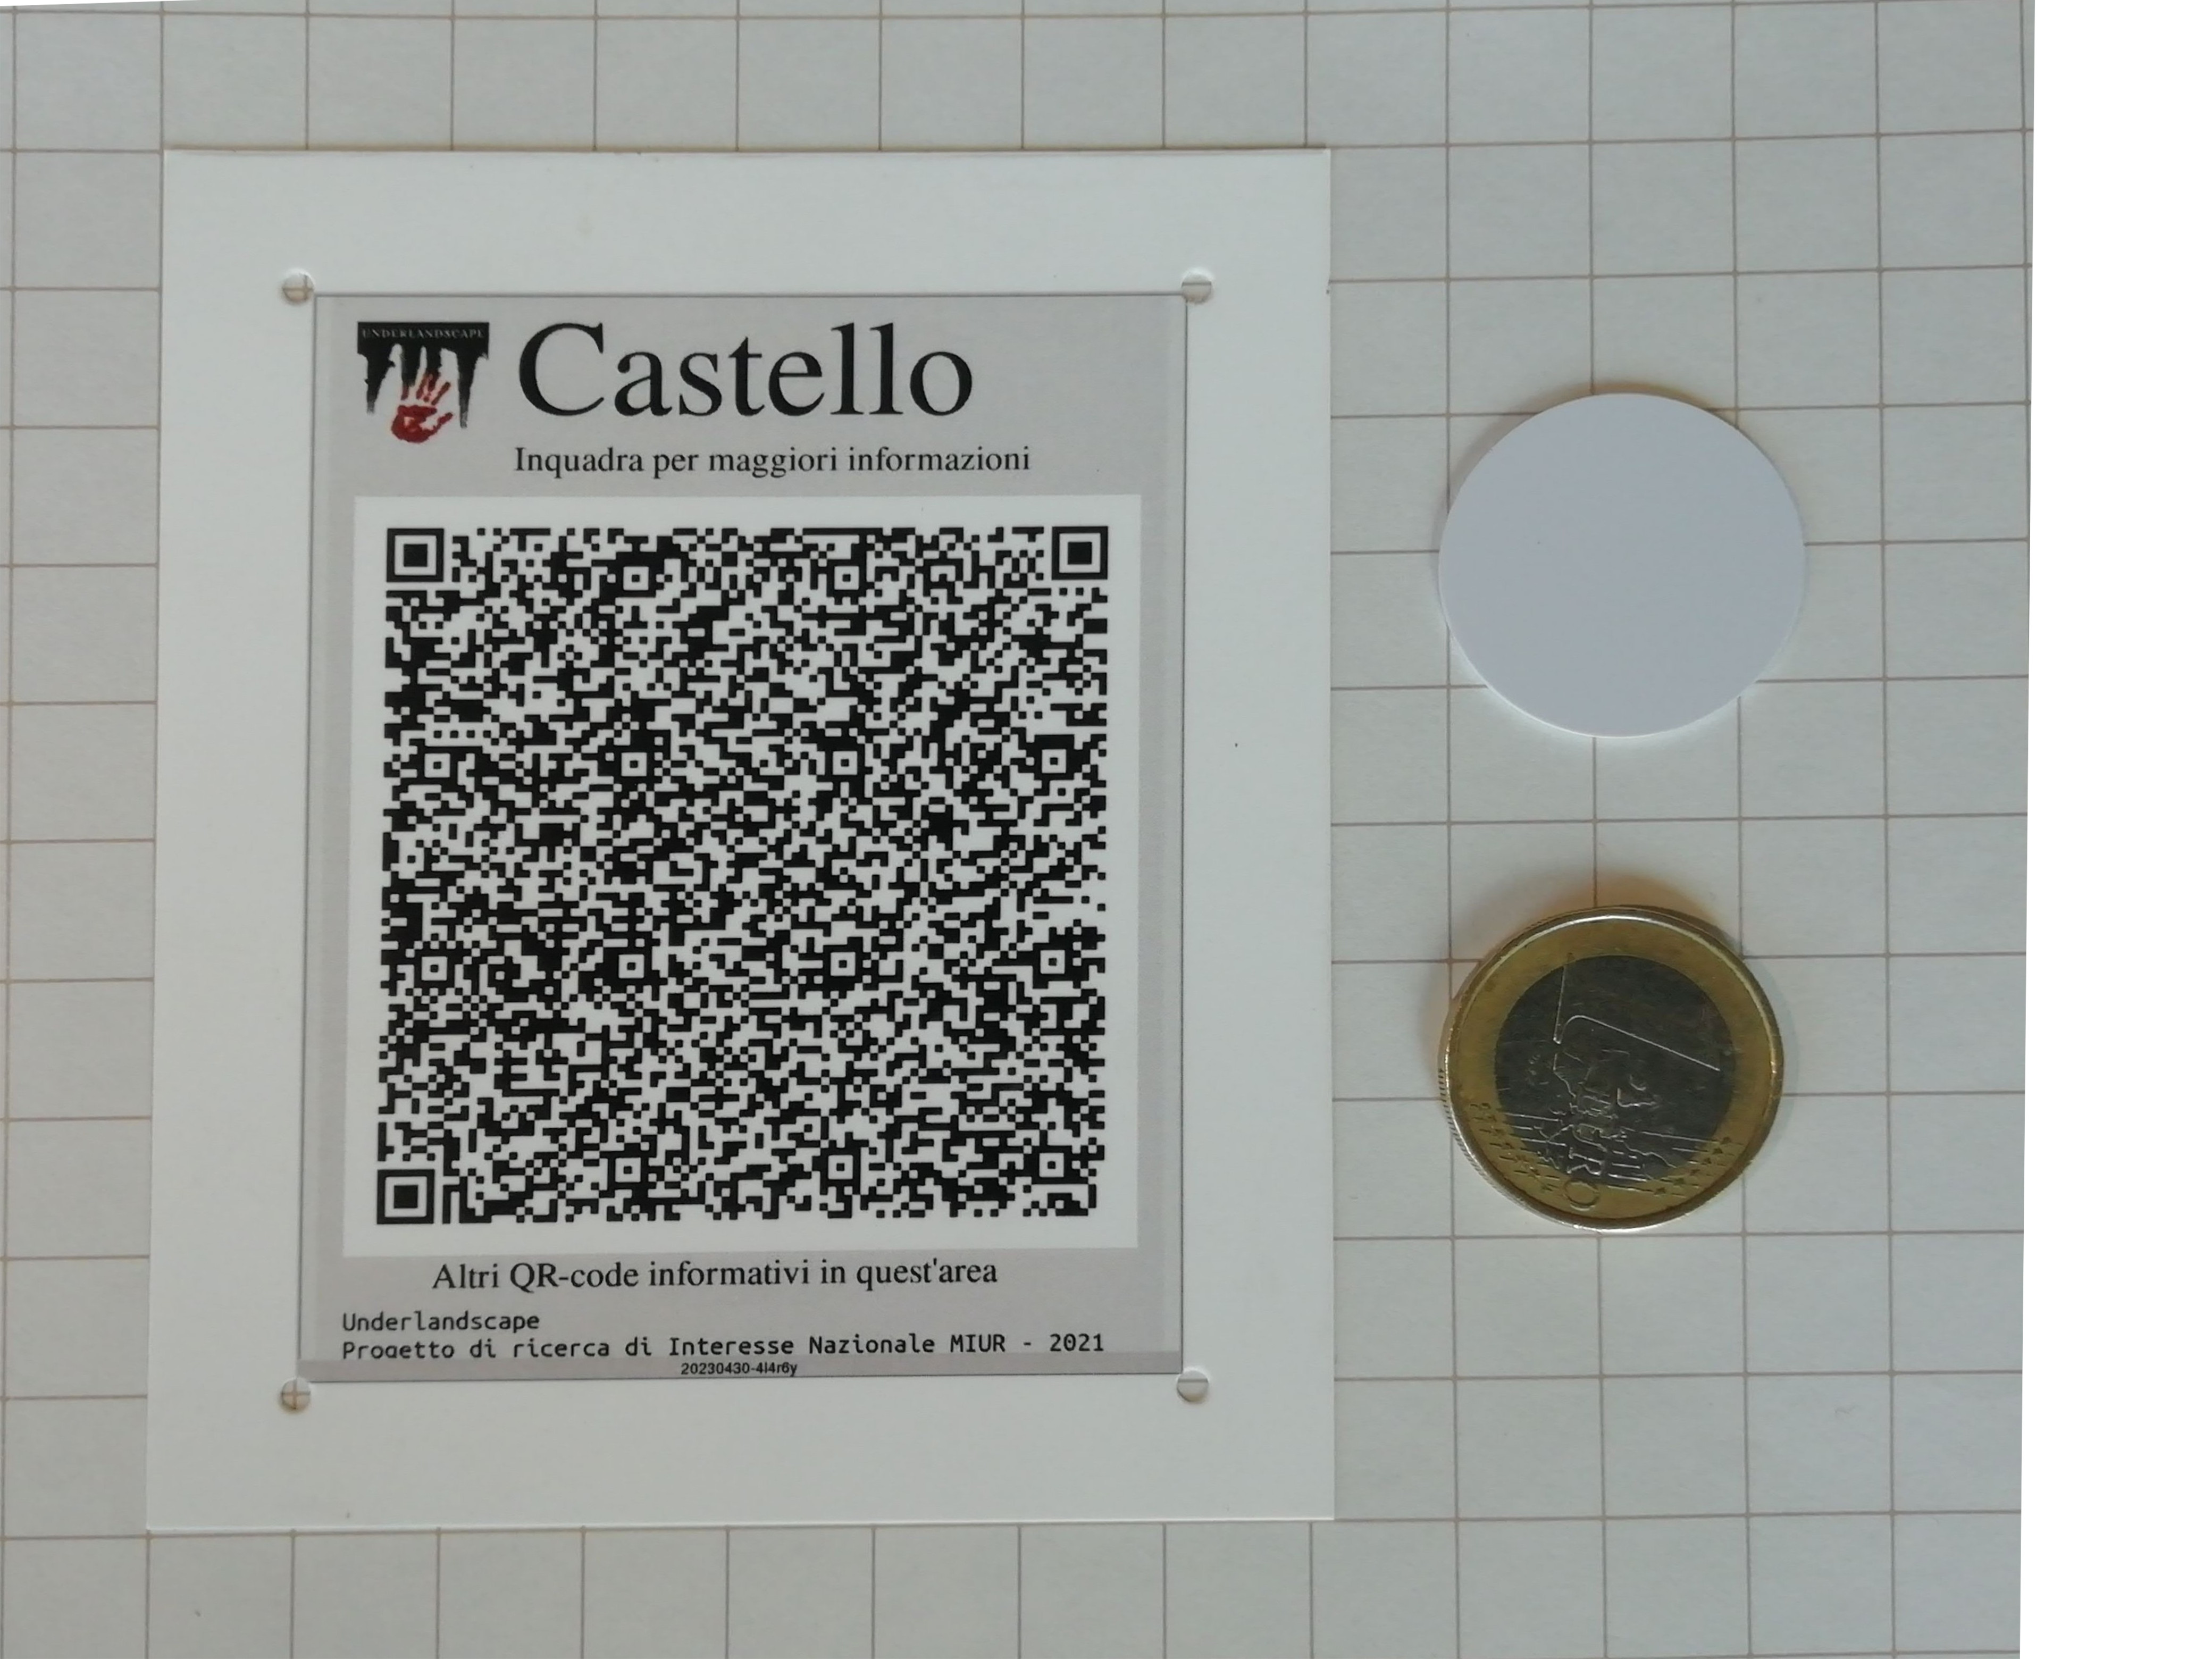
\includegraphics[width=0.9\linewidth]{figure/qr+NFC+coin}
	\caption[Passive devices dimensions]{An NFC coin, a QR-code card used in the project, and a 1 Euro coin by comparison on a paper with a square of 1cm}
	\label{fig:qrnfccoin}
\end{figure}

A preliminary check verifies compliance with the Universal Design Principles \cite{udi97a}:

%\begin{enumerate}
%	\item Equitable Use
%	\item Flexibility in Use
%	\item Simple and Intuitive
%	\item Perceptible Information
%	\item Tolerance for Error
%	\item Low Physical Effort
%	\item Size and Space for Approach and Use
%\end{enumerate}

%The labels are self-descriptive, and we address the reader to the discussion in the referenced document for a more detailed explanation.
%Checking passive devices solutions against the Universal Design principles, we assess their accessibility.

\begin{itemize}
	\item {\em Equitable use} is tighly related to the smartphone technology, which is itself considered a vehicle for equitability,
	\item {\em Flexibility in use} is enabled by the computing capabilities of the device, which allows listening to the info instead or reading, translating the information in a different language, or storage for later use,
	\item {\em Simple and intuitive use} holds since the operation requires a single application, possibly already installed since useful in many circumstances, and tag reading requires a single touch
	\item{\em Perceptible information} is a critical requirement, which contrasts with the aim of keeping low the environmental intrusion. This point will be further discussed in the section devoted to the implementation
	\item{\em Tolerance for error}: there are no margins to use the device in a way that compromises user safety. The deliberate or accidental release of the passive device into the environment determines a minor pollution
	\item{\em Low physical effort} holds, although the user needs to carry the smartphone
	\item{Size and Space for approach and use} have to be carefully considered. In the case of the NFC the smartphone needs to be nearly in touch with the passive device, while the QR-code must be in line of sight and frameable without effort
\end{itemize}

Such minimalistic solutions (see figure \ref{fig:qrnfccoin}) compares well with other solutions that make use of the user's smartphone. There is a trade-off concerning capacity, but in many circumstances a capacity of 2-300 words is sufficient to convey the description of the site, or provide directions for the the visit. If capacity limits are not an issue, a solution based on NFC or QR-codes exhibits a number of advantages:
\begin{itemize} 
\item does not require any power supply
\item has a limited impact on the landscape
\item does not entice theft
\item has a negligible cost
\item is durable
\item produces a limited quantity of waste when disposed
\item content can be stored for usage when the user reaches a zone covered by the Internet
\end{itemize}

The two passive technologies of choice exhibit the following features, that may make one of them preferable for a specific application:

\begin{itemize}
	\item an NFC-tag is smaller than a QR-tag
	\item writing an NFC-tag requires a smartphone, while the QR-tag needs a printer
	\item reading an NFC-tag operates at near-to-contact distances, while QR-codes can be read from meters away
\end{itemize}

%It significantly outperforms any active device, except for the capacity, and the NFC compares favorably only when capacity and size are prominent.

For a signage application the QR-tag is preferable because a noticeable size is needed. In addition, keeping the tag out of reach prevents vandalisms and misuse.  

In conclusion, we have reasons to select a QR-code based solution as a good candidate for a smartphone-based signage. We now consider how it it copes with the limits of a traditiona board-based approach (as listed in table \ref{tab:board}):

%The adoption of passive devices compares favorably with traditional boards, considering the strengths and limits as listed above.

\begin{itemize}
	\item dimensions: a 2-300 characters QR-code has a dimension in the order of 100 $cm^2$
	\item logistics: QR-code board can be installed on any sort of pre-existent or natural support
	\item impact: the board has a minimal interference with the landscape and may easely go un-noticed if not properly advertised
	\item accessibility for the visually impaired: the text can be read aloud
	\item international: the text can be translated
	\item update: the board can be easely replaced when the content becomes obsolete
	\item disposal: the card releases a limited quantity of pollutants related with ink support (paper or plastic)
\end{itemize}
		
%One of the issues the host must resolve is the availability of support for electronic devices. The provisioon of such support has a footprint that ha		
%may be present, but, in the spirit of our investigation, power supply should be address renewable sources, like wind, sunlight and similar.
%One option discriminates the use of an electronic device on the side of the user. 
%In case we assume the user does not have a electronic device with her, the 
%One option is to introduce active electronics: the touristic site administration provides a 
		
There are two relevant trade-offs that the host needs to resolve. One is related with the visibility of the tag. The trade-off is among visuali impact, and visibility.

Il secondo?

\section{Materials and Methods}

As anticipated in the introduction, our study wants to provide a proof of concept for a sustainable solution in a concrete setup. To comply with such an holistic approach, we need to start from the definition of the operation context.

This section is devoted to the description of the economical and social context where we are going to operate, as well as the historical backgound representing the heritage resource we want to promote. Next we will discuss the technical detail of the solution.

The geographical area of interest are the surroundings of Casoli, a small village in a mountaineous region in the north of Tuscany, in Italy. The area fall within the municipailty of Bagni di Lucca, in the province of Lucca. The archaeological team of our project formerly realized the municipal archaeological map in 2021 \cite{letizia2021}, thus assessing the reasons of interest for the heritage and the geomorphological features of the area.

\subsection{The natural and cultural resources of Casoli and its vicinity}

Bagni di Lucca is located on the north-eastern boundary of the Province of Lucca, in Val di Lima, and is part of the Media Valle del Serchio district. With its mountains it marks the historical border with the Modena and Pistoia area, it is very rich in potential for its naturalistic, archaeological and historical heritage, both expressed and as yet unexpressed. Thanks to the archaeological map the main sites of interest from prehistoric to contemporary times in this municipality are catalogued, photographed and georeferenced.

From a historical-geographical point of view, this area is identified with the Lima stream and its tributaries, that impress to the area a particular geomorphology, very impervious despite the modest hilly elevations.

The Lima stream has characterised the history of Bagni di Lucca since ever: some of the oldest evidence of human presence in the valley has
been found along its ancient river terraces, such as caves and rock shelters frequented since the Palaeolithic age; the
manufacturing industry (paper mill, flour mills and, in recent times, energy production) have exploited the since the Middle Age until the 1980s \cite{men76, bed05, ser21}.
 
On the naturalistic side, the region of Bagni di Lucca encompasses an incredible concentration of biodiversity, counting no less than three sites of the Natura 2000 Network \cite{natura2000} European Economic Community (EEC) initiative.

There are three SCIs-SACs (Sites of Community Interest and Special Areas of Conservation) located in the area north of the Lima stream, corresponding to the Apennine portion, covering 23\% of the municipal surface:
\begin {itemize}
\item the limestone areas of Val di Lima and Balzo Nero; 
\item Monte Prato Fiorito-Monte Coronato-Valle dello
Scesta; 
\item Orrido di Botri.
\end{itemize}

\begin{figure}
	\centering
	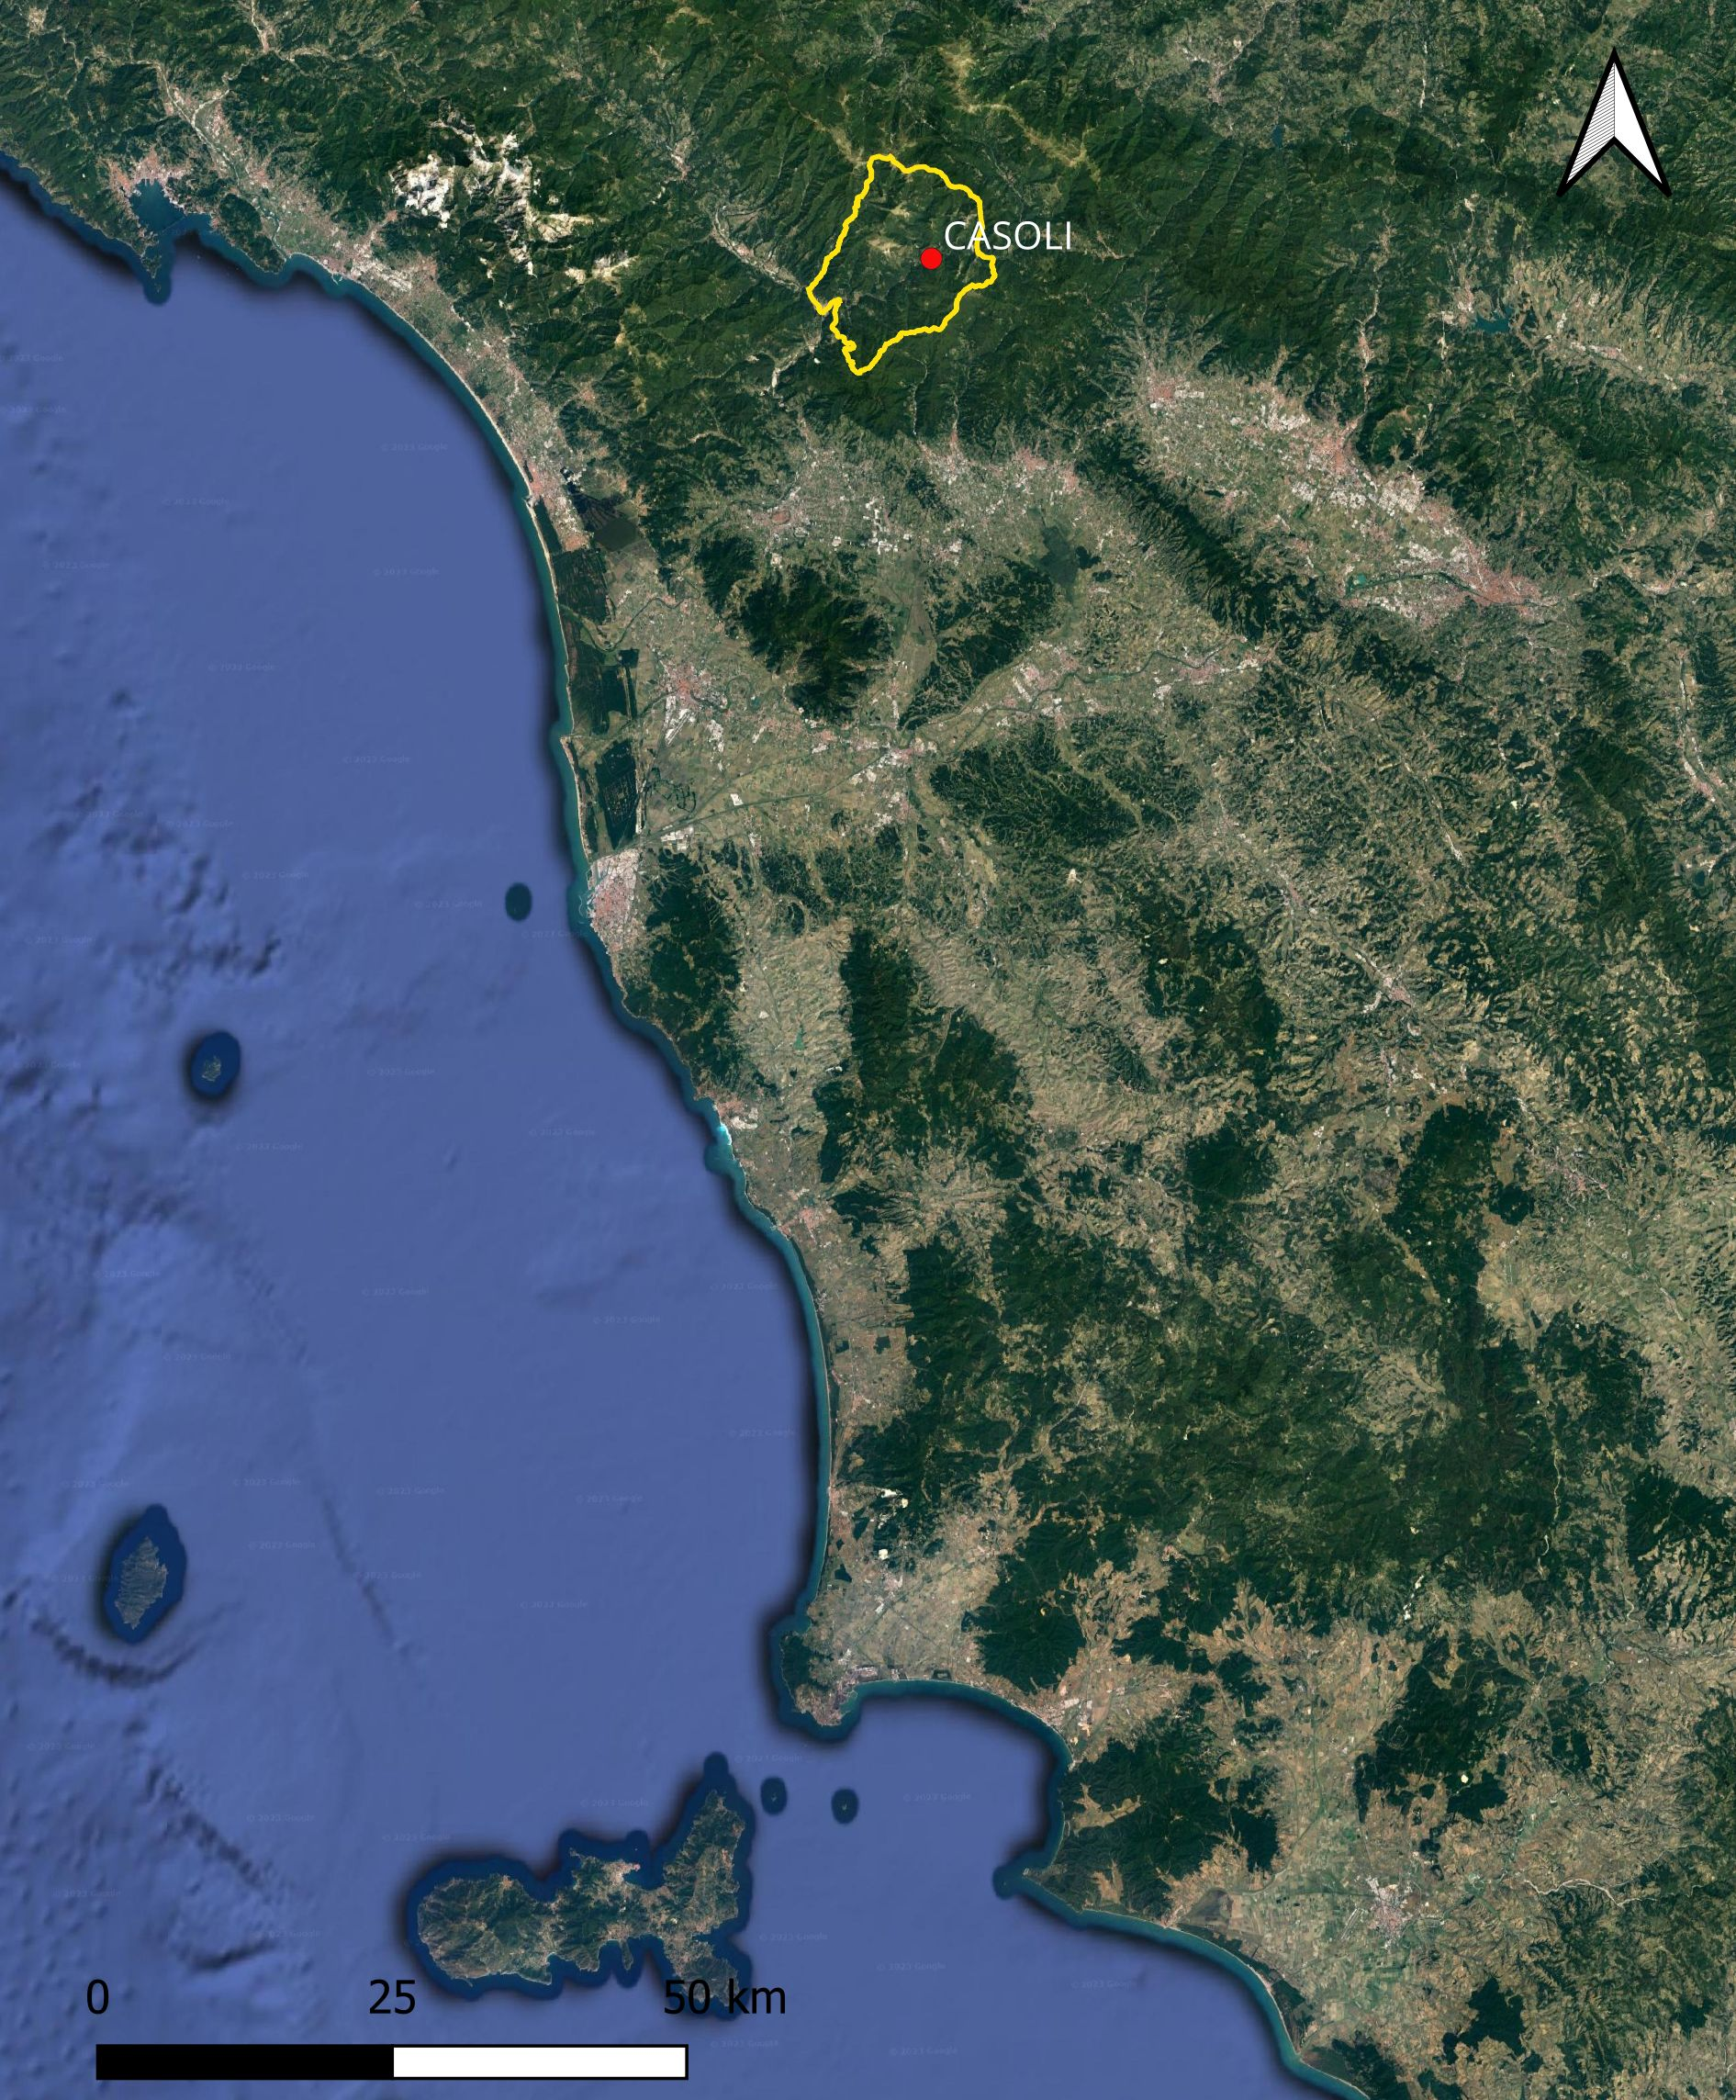
\includegraphics[width=0.3\linewidth]{figure/toscana-casoli}
	\caption[The region of Casoli]{}
	\label{fig:toscana-casoli}
\end{figure}


The latter is also a SPA (Special Protection Area) and the Orrido di Botri State Reserve is located within it \cite{nat00}. It is therefore a natural heritage with a fragile balance that needs to be preserved.

In recent years, the main tourist attractions have concentrated on the Lima stream, with some associations and private entities promoting outdoor experiences, particularly fluvial sports, such as canyoning, rafting and sup. Others important tourist attraction are trekking and hiking, supported by a network of path tracked by local CAI (Club Alpino Italiano).

In recent years the community opened two entirely new trails:
\begin{itemize}
	\item the Alta Via dei Pastori (2019), a ring around Monte Prato Fiorito that takes up the ancient grazing route, and
	\item t the Sentiero degli Avi (2020), a ring that from Montefegatesi
	reaches Monte Coronato \cite{pin21}
\end{itemize}

Another recently developed project (2019) is the expansion of the Saint Bartholomew's Path, which runs through the territory of Pistoia, with a
variant that from Popiglio continues in five stages in the municipality of Bagni di Lucca to Pieve di Controne, acting as the 'Lucca gateway' to the Path \cite{camsb}.

Such initiatives led to a considerable revival of interest among Italian and international hikers for the area, especially for the Apennine side of the valley.

We see the opportunity to improve the valorisation and enjoyment of this area by applying a slow tourism approach and involving the community, especially in the southern part of the municipality, which is still little frequented, more hilly and therefore less travelled by the trail network. We propose the creation of geo-itineraries characterised by the rediscovery of the historical roads, partly well-preserved, which connected the villages with the valley bottom and between them, including those sites of interest that encapsulate the history of this area, starting with the caves.

\subsubsection{An historical perspective of an italian mountain site}

% The village of Casoli is located on the Lima stream. To the south-east of the settlement lies a modest relief with a small glacial lake. The name of the hill ({\em "Tanette", in italian small lair} reveals the presence of karstic cavities, some inhabitated between the Paleolithic and the Iron Age . These frequentations can be attributed to a seasonal exploitation of resources and, later, with the climatic improvement, as stations on the trans-Apennine routes \cite{men76, gia96, pal63, zec72a, zec72b}.

South-east of the today location of Casoli lies a modest relief and a small glacial lake. The name of the hill ({\em "Tanette", in italian small lair} reveals the presence of karstic cavities, some inhabitated between the Paleolithic and the Iron Age and used also as stations on the trans-Apennine routes \cite{men76, gia96, pal63, zec72a, zec72b}.

Ceramic fragments dated between the 3rd century B.C. and the 1st-2nd century A.D. prove that Ligurian populations occupied the region scattered and in small nuclei. The dedication of the Latin colony of Lucca in 180 B.C. marked a decisive turning point in the Romanisation of the area and, shortly after, the definitive subjugation of the Ligurian populations, accompanied by a rapid acculturation \cite{gia96, cia05}.

We have little evidence of settlements in the mountainous hinterland, and the scarce archaeological traces are concentrated in the cave of Buca La Piella, investigated in 1975 by the Centre for Archaeological Studies of Lucca; it has two entrances joined by a walkable tunnel and rooms of discrete dimensions that overlook the outside. In addition to numerous faunal remains and fragments of locally produced common pottery, twenty bronze coins belonging to the 3rd century AD, bronze and lead objects were found. 

% Just outside the Casoli settlement, ceramic fragments datable between the 3rd century B.C. and the 1st-2nd century A.D. emerged from an excavation for the construction of a bowling green, testifying, together with other documented evidence in the area of Bagni di Lucca, how Ligurian populations settled in Val di Lima at least from the 3rd century B.C. onwards.

% In this period, the settlement must have been rather scattered and in small nuclei. The dedication of the Latin colony of Lucca in 180 B.C. marked a decisive turning point in the Romanisation of the area and within a few years there was a definitive subjugation of the Ligurian populations, accompanied by a rapid acculturation \cite{gia96, cia05}.

% From the data currently available, it can be stated that the mountainous hinterland retained a relatively marginal role. Archaeological traces for the Roman era are scarce, apart from the material that emerged from Buca La Piella, located east of Casoli along the Solco del Monte.

%The cave was discovered and investigated in 1975 by the Centre for Archaeological Studies of Lucca; it has two entrances joined by a walkable tunnel and rooms of discrete dimensions that overlook the outside. In addition to numerous faunal remains and fragments of locally produced common pottery, twenty bronze coins belonging to the 3rd century AD, bronze and lead objects were found.

% This confirms a rarefied or seasonal frequentation with a possible division in “fundi”, probably linked to the exploitation of the mountain's natural resources, the products of the forest and pasture, as well as having represented a connection route with the Po Valley area, through the Apennine passes \cite{gia96, men81, cia03}.

In addition to the scarcity of archaeological remains, there is a profound silence in the historical and literary sources for the Val di Lima from Roman and Late Antique times, although it can be assumed that the Val di Lima followed the fate of the city of Lucca, first with the occupation of the Goths and the brief Byzantine rule and then with the Longobard invasion and the formation of the Duchy of Lucca. In the hinterland, the Lombard settlement was concentrated according to a system consisting of castles and villages, mostly evidenced by documents from the 8th and 9th centuries and the remains of burial areas. In Longobard and Carolingian times, Lucca's Val di Lima was one of the three administrative districts into which the mountains were divided and was called “fines Contronenses” \cite{qui02, cia06, cia11}.

The only find from this period is the Grotta di Arzale, also known as the 'Grotta Murata', a rock shelter that opens up in the locality of Sevilucchio, north-west of Casoli along a historic road connecting Cocciglia to Casoli. Fictile artefacts, defined as being from the 'barbarian' era, have been found here; in reality, the bibliographic and oral sources collected have indicated fragments of an olla with threading, the attestation of which in the archaeological contexts of Lucca and northern Tuscany starts from the 6th-7th century and may reach as far as the end of the 11th century \cite{gia96}.

The first attestation of the settlements of Casoli and Lacu (Lake) (around the area of the Lake Casoli) dates back to the 10th century, the communities of which appear to belong to the parish of Vico Pancellorum. In this period, Bagni di Lucca was subdivided into four plebates, to which numerous villages were attached \cite{bar41, gia96}. The demographic and material entity of these agglomerates are rather elusive, but they testify to a wide-ranging distribution of the settlement with a strengthening of the social function of the churches as seats of aggregation of the population. Most documents show a widespread allivation by the bishop of Lucca of many properties, tithes, annuities and offerings of the parishes, a practice that incentivised the fractioning and alienation of ecclesiastical property in favour of certain members of the city aristocracy. In this way, they secured an accumulation of funds and power, heritages that were to the nucleus of the wealth of the future lords over the following centuries, until they emerged in
the territory by building their castles and constructing seigniorial domains centred on these areas \cite{qui02, gia96, for12, for15}.

Written sources mention a castle in Casoli from 1180, the year in which the fortification is in the hands of the Bishop of Lucca, but its foundation must be earlier, probably built during the 11th- 12th centuries. It occupies the summit of Colle delle Tanette, towering to the north of the village.

Between the 13th and 15th centuries, the fortification was at the centre, along with the other castles of the Val di Lima, of clashes between Lucca, Pisa and Florence, with alternating fortunes, as it was a strategic border area for the power of Lucca. Today, very little is preserved and the area has been partly inhabited. The fortified complex must have been equipped with
two walls, a tower on the highest portion of the hill that is poorly preserved and two buildings.

According to some oral sources, part of the castle stones were re-used to construct the surrounding buildings \cite{gia96, for12, rom16}. The same document from 1180 mentions the church of San Donato, located in the main square on the north-western edge of the village of Casoli. The current structure dates back to the 12th-13th centuries, with subsequent renovations and an enlargement of the naves that partially incorporated the base of the bell tower. The façade is surmounted by a plastered moulded tympanum, while the side aisles are adorned with moulded cornices. Initially dedicated only to San Donato, it acquired the double dedication after the abandonment of the church of Sant'Andrea de Lacu. The latter is located on a plateau to the east of Lake Casoli and is attested from 1260 in the Estimi of the diocese of Lucca as being subject to the parish of Vico Pancellorum \cite{ber18, gia96, cap17}, but already from the pastoral visit of 1358 it appears to have been united to the church of Casoli and from the pastoral visit of 1467 we learn of its state of abandonment \cite{gia96, con12}. This was probably due to the depopulation of the lake area and the simultaneous strengthening of the town of Casoli, which was fortified and better protected during this unstable phase.

Today, the romanesque church of Sant'Andrea de Lacu is in a state of decay, with a rectangular plan, ending on the east side with a semi-circular apse; the masonry is characterised by squared lithic blocks arranged in regular rows. Inside, there is a reused element of the previous building walled into the northern perimeter, testifying to an older origin, probably contemporary with the settlement of Lacu (Lake) mentioned in sources from the 10th century and no longer visible today.

Nearby are the remains of a quadrangular building with masonry in lithic blocks arranged in fairly regular rows, dating back to the Middle Ages (13th century), possibly a residential building.

In the early modern age, villages that survived the demographic crisis of the 14th-15th centuries experienced a progressive architectural renewal between the 16th and 18th centuries, which still largely characterizes the settlements today. Within Casoli, a series of residential buildings with imposing dated portals are preserved, some with courtyards, and mansions that denote a discrete deployment of resources by wealthy social classes. There is also a well-preserved bread oven, typically used by the entire community, which remained in use at least for village festivals until a few decades ago.

Two oratories in the village date back to the modern age (17th-18th centuries): one dedicated to the Madonna of Loreto, flanked by a wash-house, and the other called Madonna di Castello and characterised by an entrance enclosure, located along the cobbled road that retraces the ancient road linking the village with the summit area of the medieval castle \cite{gia96}.

Casoli was connected to the valley floor by two main roads attested in the Borbonic Cadastre, which from the village follow the gentler slopes to the east and south-west to ford the Lima torrent thanks to the Ponte Maggio and Ponte Nero bridges, still preserved today. Towards the hilly area, an articulated road network is evidenced, which is still legible in the landscape and in part is taken up by the CAI trail system. In particular, from the village starts the road that led toward Lucchio crossing the area of Casoli Lake. Along it are the chapel of Madonna di Col di Piano and two “metati” referable to the contemporary age, used for drying chestnuts. The entire area of the lake is covered with crops of centuries-old chestnut trees, typical of the Lima Valley, as of the entire Apennine area. Referred to as the "bread tree," chestnut fruits and the flour derived from them were a staple of the mountain diet until the mid-1900s, and today they are increasingly less common due to the disease that has affected their specimens and the slow replacement by allochthonous species \cite{buc92, puc10}.

\subsubsection{The socio-economical context of Casoli and its vicinity}

......

\subsubsection{Sites and trail’s state of art}

%The study of the Casoli area made it possible to identify the historical-archaeological sites considered of greatest interest for the purposes of a geotouristic route. Once these sites had been located and the possible paths to reach them analysed, also by consulting the online sharing of itineraries by hikers and climbers, we carried out field surveys between April and June 2023 to check the status of the trails and sites for their enjoyment. (questo penso di metterlo dopo)

As explained in the previous section, the area around Casoli has a long history witnessed by architectural and geological features: it is therefore a good candidate for our case study. In the rest of this section we define the features of interest, and report about their accessibility.

%The site at the centre of the project's interest is Buca La Piella, a cave located along the Solco del Monte and off the conventional circuits, which is why it is less frequented and consequently less compromised for the scientific analyses that will be carried out there, compared to the caves located along the Lima stream, near the state highway. The first part of the route coincides for about 500 m with CAI path 386, which together with path 388 forms the Casoli-Lucchio ring around Monte Memoriante. Access to the path, which is poorly marked with a faded red and white simple signpost, is along the asphalt road that leads from Ponte Maggio to Casoli and starts from the slope with a short stone ramp. After a short climb, one walks at altitudealong the slope and then enters the forest, skirting the final part of the Solco del Monte, known as Rio di Castello.

The cave named {\em Buca La Piella} is the foremost site from an archeological point of view. It is located in a fascinating environment outside conventional circuits, which is why it is less frequented and consequently less compromised. It is reachable leaving a marked path to follow the bed of the Lima river. The way is dotted with minor karsic caves, and the {\em Buca La Piella} is reachable climbing up on a steep slope in the wood on the right of the Lima river. 

%A faint track through the grass diverts from the path to climb up the side of the slope to the rock face where one of the many karstic formations that characterise the area opens up. This is a small cave, called the 'Antro dell'Ugola' in the Tuscan speleological register. It consists of two openings whose entrance has a conformation reminiscent of a uvula. There are no proven finds, but the space inside and the position could indicate a frequentation that will be verified with the comparison analyses that we will carry out.

Not far from the {\em Buca La Piella} on the same side of the river is another karst cave named {\em Antro dell'Ugola}. It is reachable following a faint and intermittent track that departs from a marked path. It is craracterize by a suspended geological formation reminding an uvula, hence the name.

Both caves are going to be analyzed in the course of the Underlandscape project \cite{Underlandscape}, and findings can further enhance the interest for both sites.

\textbf{Qui aggiungerei notizie sugli altri punti in cui sono stati collocati i QR-code, correlandoli alla descrizione storica
}

%We return to the main path, this one looking over the Rio to proceed in the direction of Lucchio, while we abandon it to penetrate between the high rock walls carved over time by the Rio; mobile network coverage is absent, while the GPS has poor coverage and in many places is unreliable. When walking along the stream bed, great care is required, due to slippery pebbles and sections with wet foliage and moss. After about 300 m, follow a track that climbs up the slope to the right. When you reach a small plateau, you will find a rock shelter, which is not marked in the Tuscan cave cadastre and has not yet been investigated. Buca La Piella is located about 120 m further north. To reach it, climb up to the rock face by crossing a rather steep wooded slope. A great deal of caution is required, and for future use it would be a good idea to at least provide a safety rope. When you reach the wall, there is a short tunnel that leads into the cave. A very wide and high cavity opens up towards the east. The vault has a hole in the centre, and there are stalactites and stalagmites. The ground descends gently towards the opening, beyond which the slope becomes steep, making it necessary in the future to secure it with nets or fences.

\subsection{Implementing a QR-based signage}

To test our signage proposal, we placed on the field several cards carrying QR codes. Se the list in Table~\ref{tab:qrtags}.

% TODO: \usepackage{graphicx} required
\begin{figure}
	\centering
	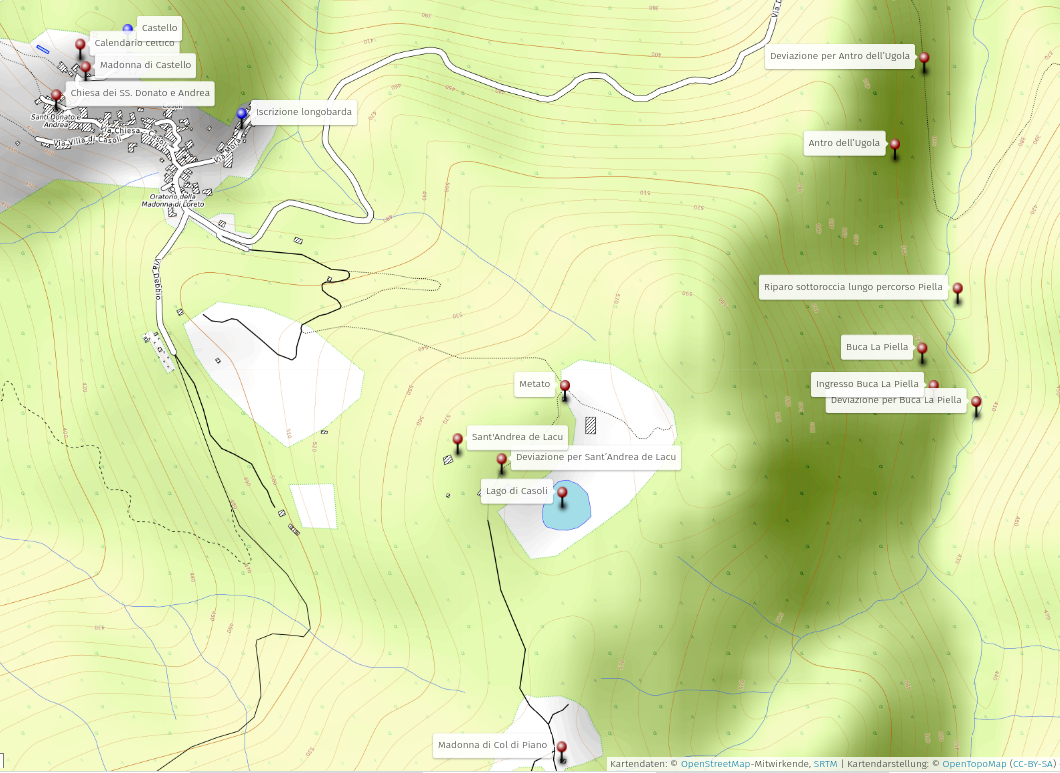
\includegraphics[width=\linewidth]{figure/mappa}
	\caption[Map with QR-tag positions]{}
	\label{fig:mappa}
\end{figure}


\begin{table}
	\begin{tabular}{|>{\raggedright\arraybackslash}p{3cm}|l|l|l|l|}
\hline 
\textbf{Name} & \textbf{Long} & \textbf{Lat} & \textbf{URL Key} & \textbf{Length} \\
\hline
Buca La Piella & 10.68361 & 44.03667 & t5ysrm & 476 \\
\hline
Calendario celtico & 10.66985 & 44.03986 & my0kp8 & 484 \\
\hline
Castello & 10.67062 & 44.04004 & 4l4r6y & 597 \\
\hline
Chiesa dei SS. Donato e Andrea & 10.66947 & 44.03928 & lwtyx6 & 632 \\
\hline
Iscrizione longobarda & 10.67244 & 44.03906 & 60m75s & 369 \\
\hline
Lago di Casoli & 10.67761 & 44.03468 & xqjpbk & 369 \\
\hline
Madonna di Castello & 10.66994 & 44.03960 & qlci89 & 395 \\
\hline
Madonna di Col di Piano & 10.67760 & 44.03173 & 3w44wr & 414 \\
\hline
Metato & 10.67764 & 44.03591 & sbgnl0 & 660 \\
\hline
Sant'Andrea de Lacu & 10.67592 & 44.03530 & fxq83v & 657 \\
\hline
Antro dell’Ugola & 10.68296 & 44.03871 & mprs0w & 226 \\
\hline
Deviazione per Antro dell’Ugola & 10.68343 & 44.03971 & e4n2js & 88 \\
\hline
Deviazione per Buca La Piella & 10.68427 & 44.03573 & hve4pj & 139 \\
\hline
Deviazione per Sant’Andrea de Lacu & 10.67663 & 44.03507 & 13uav3 & 200 \\
\hline
Ingresso Buca La Piella & 10.68358 & 44.03592 & 5ahvp8 & 190 \\
\hline
Riparo sottoroccia lungo percorso Piella & 10.68397 & 44.03704 & kwr1wx & 286 \\
\hline
	\end{tabular}
\caption{The QR-tags placed around Casoli. The URL key is a random code that appears in the web page linked to the QR code. The Length refers to the description in the QR-code and is in characters. \label{tab:qrtags}}
\end{table}

A card sample is in Figure \ref{fig:toscana-casoli}. On the top there is the logo of the funding project, a descriptive title ({\em Castle} in english) and concise directions for use {\em Scan fo further information}). Under the QR-code is the notice that other QR-codes are present in the vicinity, and a reference to the funding project.

The text in the QR-code (in figure \ref{fig:qrcodecontent}) contains the main text with 614 characters (100 words) and a URL 86 characters long. The URL is useful only if the Internet is reachable, and brings to a new page containing a map with the location of all the tags (Figure \ref{fig:linkmap}) and a short survey form. Note that, while the QR-tag content is always available, the URL is reachable in locations with broadband coverage. In our case, during a recon to the {\em Piella} cave none of the smartphones of the participants received sufficient broadband network signal.

\begin{figure}
\subfloat[QR-tag content]{
	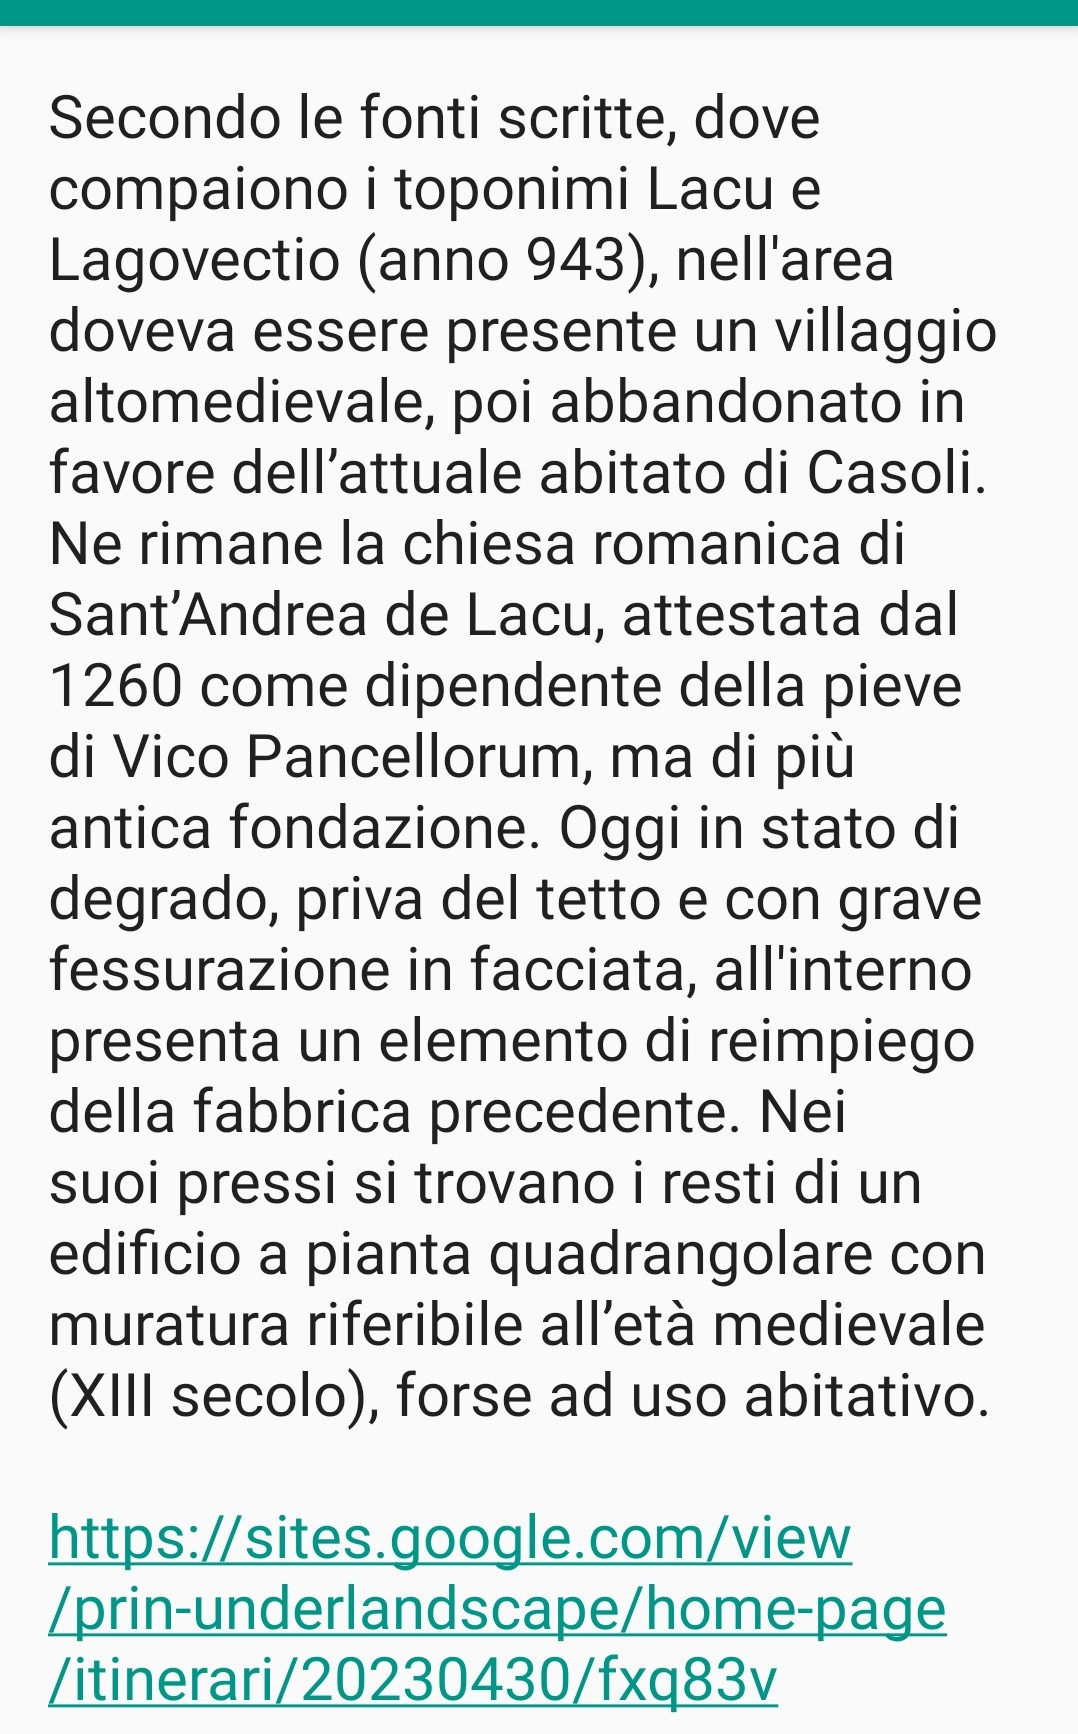
\includegraphics[width = 0.3 \linewidth]{figure/qr-code-content}
	\label{fig:qrcodecontent}
}
\subfloat[Linked page: the map]{
	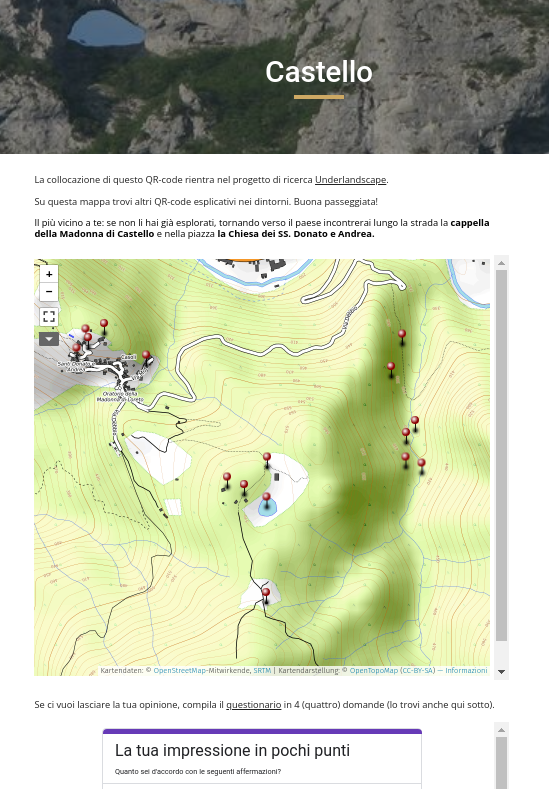
\includegraphics[width = 0.3 \linewidth]{figure/sito-a}
	\label{fig:linkmap}
}
\subfloat[Linked page: survey form]{
	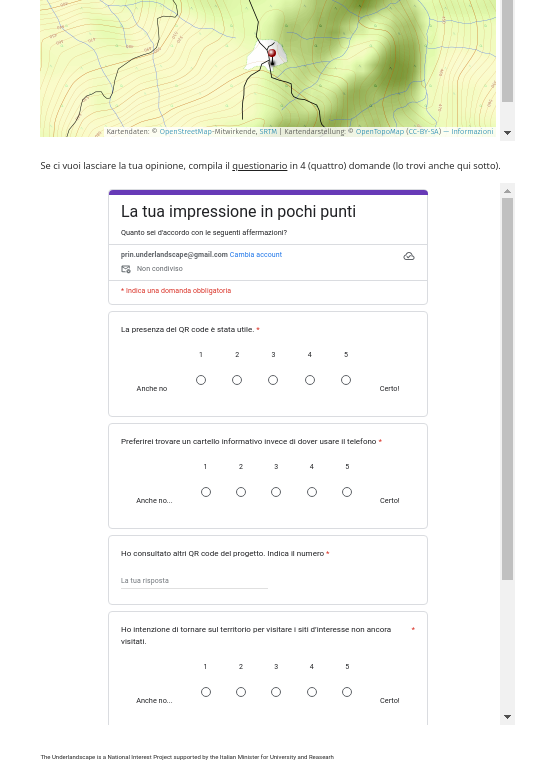
\includegraphics[width = 0.3 \linewidth]{figure/sito-b}
	\label{fig:linksurvey}
}
\end{figure}


We placed QR-tags both along the trail and at sites of interest; the former are placed at detours and, at more complex points, at close range so that from one you can see the next, as per the CAI standard \cite{cai10}.

They can therefore have either the function of a simple signpost to indicate the continuity of the trail, or be scanned to read the written indications recorded within it, which are more accurate and precise. 

%QR codes placed at sites of interest provide historical, archaeological and naturalistic information through short text descriptions. They also give the possibility, where phone coverage allows, to deepen the project and discover more details about the proposed itinerary through a link to the dedicated site.

This approach ensures that the tourist is guided through the visitor experience and, at the same time, that the impact of signage on the environment is reduced compared with traditional boards, as explained in section \ref{sec:minimize}.

%, considering that there is no need for panels and vertical signage involving the placement of poles. In addition to being more impactful, classic vertical signage can more easily suffer degradation and needs more maintenance, especially the information paneling on the sites; whereas in our proposal the possible maintenance of the QR code would constitute very short time and rather low cost.

Clearly, our methodology does not aim to replace CAI signage, which is recognized throughout the country and is very effective, especially in terms of horizontal typology, but at the very least it is repurposed to complement it in order to provide more detailed information at multiple levels of interest, from short text to in-depth information on the project site. In addition, being able to read the written directions along the path can be of great help to even the most inexperienced hikers, particularly on unclear and not-quite-visible trails such as the one we suggested to reach Buca La Piella.


% ====




% Concentrate on outdoor activities


% Starting from previous experiences documented in the bibliography we explore a few broad categories, to find weaknesses and strengths for each of them.

% One of the issues the host must resolve is the availability of support for electronic devices. The provisioon of such support has a footprint that ha

% may be present, but, in the spirit of our investigation, power supply should be address renewable sources, like wind, sunlight and similar.

% One option discriminates the use of an electronic device on the side of the user. 

% In case we assume the user does not have a electronic device with her, the 
% One option is to introduce active electronics: the touristic site administration provides a 


%Materials and Methods should be described with sufficient details to allow others to replicate and build on published results. Please note that publication of your manuscript implicates that you must make all materials, data, computer code, and protocols associated with the publication available to readers. Please disclose at the submission stage any restrictions on the availability of materials or information. New methods and protocols should be described in detail while well-established methods can be briefly described and appropriately cited.

%Research manuscripts reporting large datasets that are deposited in a publicly avail-able database should specify where the data have been deposited and provide the relevant accession numbers. If the accession numbers have not yet been obtained at the time of submission, please state that they will be provided during review. They must be provided prior to publication.

%Interventionary studies involving animals or humans, and other studies require ethical approval must list the authority that provided approval and the corresponding ethical approval code.
%\begin{quote}
%This is an example of a quote.
%\end{quote}

%%%%%%%%%%%%%%%%%%%%%%%%%%%%%%%%%%%%%%%%%%
\section{Results}

%This section may be divided by subheadings. It should provide a concise and precise description of the experimental results, their interpretation as well as the experimental conclusions that can be drawn.
%\subsection{Subsection}
%\subsubsection{Subsubsection}

%Bulleted lists look like this:
%\begin{itemize}
%\item	First bullet;
%\item	Second bullet;
%\item	Third bullet.
%\end{itemize}

%Numbered lists can be added as follows:
%\begin{enumerate}
%\item	First item; 
%\item	Second item;
%\item	Third item.
%\end{enumerate}

%The text continues here. 
%
%\subsection{Figures, Tables and Schemes}
%
%All figures and tables should be cited in the main text as Figure~\ref{fig1}, Table~\ref{tab1}, etc.
%
%\begin{figure}[H]
%
\includegraphics[width=10.5 cm]{Definitions/logo-mdpi}
%\caption{This is a figure. Schemes follow the same formatting. If there are multiple panels, they should be listed as: (\textbf{a}) Description of what is contained in the first panel. (\textbf{b}) Description of what is contained in the second panel. Figures should be placed in the main text near to the first time they are cited. A caption on a single line should be centered.\label{fig1}}
%\end{figure}   
%\unskip
%
%\begin{table}[H] 
%\caption{This is a table caption. Tables should be placed in the main text near to the first time they are~cited.\label{tab1}}
%\newcolumntype{C}{>{\centering\arraybackslash}X}
%\begin{tabularx}{\textwidth}{CCC}
%\toprule
%\textbf{Title 1}	& \textbf{Title 2}	& \textbf{Title 3}\\
%\midrule
%Entry 1		& Data			& Data\\
%Entry 2		& Data			& Data \textsuperscript{1}\\
%\bottomrule
%\end{tabularx}
%\noindent{\footnotesize{\textsuperscript{1} Tables may have a footer.}}
%\end{table}
%
%The text continues here (Figure~\ref{fig2} and Table~\ref{tab2}).
%
%% Example of a figure that spans the whole page width. The same concept works for tables, too.
%\begin{figure}[H]
%\begin{adjustwidth}{-\extralength}{0cm}
%\centering
%
\includegraphics[width=15.5cm]{Definitions/logo-mdpi}
%\end{adjustwidth}
%\caption{This is a wide figure.\label{fig2}}
%\end{figure}  
%
%\begin{table}[H]
%\caption{This is a wide table.\label{tab2}}
%	\begin{adjustwidth}{-\extralength}{0cm}
%		\newcolumntype{C}{>{\centering\arraybackslash}X}
%		\begin{tabularx}{\fulllength}{CCCC}
%			\toprule
%			\textbf{Title 1}	& \textbf{Title 2}	& \textbf{Title 3}     & \textbf{Title 4}\\
%			\midrule
%\multirow[m]{3}{*}{Entry 1 *}	& Data			& Data			& Data\\
%			  	                   & Data			& Data			& Data\\
%			             	      & Data			& Data			& Data\\
%                   \midrule
%\multirow[m]{3}{*}{Entry 2}    & Data			& Data			& Data\\
%			  	                  & Data			& Data			& Data\\
%			             	     & Data			& Data			& Data\\
%                   \midrule
%\multirow[m]{3}{*}{Entry 3}    & Data			& Data			& Data\\
%			  	                 & Data			& Data			& Data\\
%			             	    & Data			& Data			& Data\\
%                  \midrule
%\multirow[m]{3}{*}{Entry 4}   & Data			& Data			& Data\\
%			  	                 & Data			& Data			& Data\\
%			             	    & Data			& Data			& Data\\
%			\bottomrule
%		\end{tabularx}
%	\end{adjustwidth}
%	\noindent{\footnotesize{* Tables may have a footer.}}
%\end{table}

%\begin{listing}[H]
%\caption{Title of the listing}
%\rule{\columnwidth}{1pt}
%\raggedright Text of the listing. In font size footnotesize, small, or normalsize. Preferred format: left aligned and single spaced. Preferred border format: top border line and bottom border line.
%\rule{\columnwidth}{1pt}
%\end{listing}

%Text.
%
%Text.
%
%\subsection{Formatting of Mathematical Components}
%
%This is the example 1 of equation:
%\begin{linenomath}
%\begin{equation}
%a = 1,
%\end{equation}
%\end{linenomath}
%the text following an equation need not be a new paragraph. Please punctuate equations as regular text.
%%% If the documentclass option "submit" is chosen, please insert a blank line before and after any math environment (equation and eqnarray environments). This ensures correct linenumbering. The blank line should be removed when the documentclass option is changed to "accept" because the text following an equation should not be a new paragraph.
%
%This is the example 2 of equation:
%\begin{adjustwidth}{-\extralength}{0cm}
%\begin{equation}
%a = b + c + d + e + f + g + h + i + j + k + l + m + n + o + p + q + r + s + t + u + v + w + x + y + z
%\end{equation}
%\end{adjustwidth}
%
%% Example of a page in landscape format (with table and table footnote).
%%\startlandscape
%%\begin{table}[H] %% Table in wide page
%%\caption{This is a very wide table.\label{tab3}}
%%	\begin{tabularx}{\textwidth}{CCCC}
%%		\toprule
%%		\textbf{Title 1}	& \textbf{Title 2}	& \textbf{Title 3}	& \textbf{Title 4}\\
%%		\midrule
%%		Entry 1		& Data			& Data			& This cell has some longer content that runs over two lines.\\
%%		Entry 2		& Data			& Data			& Data\textsuperscript{1}\\
%%		\bottomrule
%%	\end{tabularx}
%%	\begin{adjustwidth}{+\extralength}{0cm}
%%		\noindent\footnotesize{\textsuperscript{1} This is a table footnote.}
%%	\end{adjustwidth}
%%\end{table}
%%\finishlandscape
%
%
%Please punctuate equations as regular text. Theorem-type environments (including propositions, lemmas, corollaries etc.) can be formatted as follows:
%%% Example of a theorem:
%\begin{Theorem}
%Example text of a theorem.
%\end{Theorem}
%
%The text continues here. Proofs must be formatted as follows:
%
%%% Example of a proof:
%\begin{proof}[Proof of Theorem 1]
%Text of the proof. Note that the phrase ``of Theorem 1'' is optional if it is clear which theorem is being referred to.
%\end{proof}
%The text continues here.
%
%%%%%%%%%%%%%%%%%%%%%%%%%%%%%%%%%%%%%%%%%%%
%\section{Discussion}
%
%Authors should discuss the results and how they can be interpreted from the perspective of previous studies and of the working hypotheses. The findings and their implications should be discussed in the broadest context possible. Future research directions may also be highlighted.
%
%%%%%%%%%%%%%%%%%%%%%%%%%%%%%%%%%%%%%%%%%%%
%\section{Conclusions}
%
%This section is not mandatory, but can be added to the manuscript if the discussion is unusually long or complex.
%
%%%%%%%%%%%%%%%%%%%%%%%%%%%%%%%%%%%%%%%%%%%
%\section{Patents}
%
%This section is not mandatory, but may be added if there are patents resulting from the work reported in this manuscript.

%%%%%%%%%%%%%%%%%%%%%%%%%%%%%%%%%%%%%%%%%%
\vspace{6pt} 

%%%%%%%%%%%%%%%%%%%%%%%%%%%%%%%%%%%%%%%%%%
%% optional
%\supplementary{The following supporting information can be downloaded at:  \linksupplementary{s1}, Figure S1: title; Table S1: title; Video S1: title.}

% Only for the journal Methods and Protocols:
% If you wish to submit a video article, please do so with any other supplementary material.
% \supplementary{The following supporting information can be downloaded at: \linksupplementary{s1}, Figure S1: title; Table S1: title; Video S1: title. A supporting video article is available at doi: link.}

%%%%%%%%%%%%%%%%%%%%%%%%%%%%%%%%%%%%%%%%%%
\authorcontributions{For research articles with several authors, a short paragraph specifying their individual contributions must be provided. The following statements should be used ``Conceptualization, X.X. and Y.Y.; methodology, X.X.; software, X.X.; validation, X.X., Y.Y. and Z.Z.; formal analysis, X.X.; investigation, X.X.; resources, X.X.; data curation, X.X.; writing---original draft preparation, X.X.; writing---review and editing, X.X.; visualization, X.X.; supervision, X.X.; project administration, X.X.; funding acquisition, Y.Y. All authors have read and agreed to the published version of the manuscript.'', please turn to the  \href{http://img.mdpi.org/data/contributor-role-instruction.pdf}{CRediT taxonomy} for the term explanation. Authorship must be limited to those who have contributed substantially to the work~reported.}

\funding{Please add: ``This research received no external funding'' or ``This research was funded by NAME OF FUNDER grant number XXX.'' and  and ``The APC was funded by XXX''. Check carefully that the details given are accurate and use the standard spelling of funding agency names at \url{https://search.crossref.org/funding}, any errors may affect your future funding.}

\institutionalreview{In this section, you should add the Institutional Review Board Statement and approval number, if relevant to your study. You might choose to exclude this statement if the study did not require ethical approval. Please note that the Editorial Office might ask you for further information. Please add “The study was conducted in accordance with the Declaration of Helsinki, and approved by the Institutional Review Board (or Ethics Committee) of NAME OF INSTITUTE (protocol code XXX and date of approval).” for studies involving humans. OR “The animal study protocol was approved by the Institutional Review Board (or Ethics Committee) of NAME OF INSTITUTE (protocol code XXX and date of approval).” for studies involving animals. OR “Ethical review and approval were waived for this study due to REASON (please provide a detailed justification).” OR “Not applicable” for studies not involving humans or animals.}

\informedconsent{Any research article describing a study involving humans should contain this statement. Please add ``Informed consent was obtained from all subjects involved in the study.'' OR ``Patient consent was waived due to REASON (please provide a detailed justification).'' OR ``Not applicable'' for studies not involving humans. You might also choose to exclude this statement if the study did not involve humans.

Written informed consent for publication must be obtained from participating patients who can be identified (including by the patients themselves). Please state ``Written informed consent has been obtained from the patient(s) to publish this paper'' if applicable.}

\dataavailability{We encourage all authors of articles published in MDPI journals to share their research data. In this section, please provide details regarding where data supporting reported results can be found, including links to publicly archived datasets analyzed or generated during the study. Where no new data were created, or where data is unavailable due to privacy or ethical re-strictions, a statement is still required. Suggested Data Availability Statements are available in section “MDPI Research Data Policies” at \url{https://www.mdpi.com/ethics}.} 

\acknowledgments{In this section you can acknowledge any support given which is not covered by the author contribution or funding sections. This may include administrative and technical support, or donations in kind (e.g., materials used for experiments).}

\conflictsofinterest{Declare conflicts of interest or state ``The authors declare no conflict of interest.'' Authors must identify and declare any personal circumstances or interest that may be perceived as inappropriately influencing the representation or interpretation of reported research results. Any role of the funders in the design of the study; in the collection, analyses or interpretation of data; in the writing of the manuscript; or in the decision to publish the results must be declared in this section. If there is no role, please state ``The funders had no role in the design of the study; in the collection, analyses, or interpretation of data; in the writing of the manuscript; or in the decision to publish the~results''.} 

%%%%%%%%%%%%%%%%%%%%%%%%%%%%%%%%%%%%%%%%%%
%% Optional
\sampleavailability{Samples of the compounds ... are available from the authors.}

%% Only for journal Encyclopedia
%\entrylink{The Link to this entry published on the encyclopedia platform.}

\abbreviations{Abbreviations}{
The following abbreviations are used in this manuscript:\\

\noindent 
\begin{tabular}{@{}ll}
MDPI & Multidisciplinary Digital Publishing Institute\\
DOAJ & Directory of open access journals\\
TLA & Three letter acronym\\
LD & Linear dichroism
\end{tabular}
}

%%%%%%%%%%%%%%%%%%%%%%%%%%%%%%%%%%%%%%%%%%%
%%% Optional
%\appendixtitles{no} % Leave argument "no" if all appendix headings stay EMPTY (then no dot is printed after "Appendix A"). If the appendix sections contain a heading then change the argument to "yes".
%\appendixstart
%\appendix
%\section[\appendixname~\thesection]{}
%\subsection[\appendixname~\thesubsection]{}
%The appendix is an optional section that can contain details and data supplemental to the main text---for example, explanations of experimental details that would disrupt the flow of the main text but nonetheless remain crucial to understanding and reproducing the research shown; figures of replicates for experiments of which representative data are shown in the main text can be added here if brief, or as Supplementary Data. Mathematical proofs of results not central to the paper can be added as an appendix.
%
%\begin{table}[H] 
%\caption{This is a table caption.\label{tab5}}
%\newcolumntype{C}{>{\centering\arraybackslash}X}
%\begin{tabularx}{\textwidth}{CCC}
%\toprule
%\textbf{Title 1}	& \textbf{Title 2}	& \textbf{Title 3}\\
%\midrule
%Entry 1		& Data			& Data\\
%Entry 2		& Data			& Data\\
%\bottomrule
%\end{tabularx}
%\end{table}
%
%\section[\appendixname~\thesection]{}
%All appendix sections must be cited in the main text. In the appendices, Figures, Tables, etc. should be labeled, starting with ``A''---e.g., Figure A1, Figure A2, etc.
%
%%%%%%%%%%%%%%%%%%%%%%%%%%%%%%%%%%%%%%%%%%%
\begin{adjustwidth}{-\extralength}{0cm}
%%\printendnotes[custom] % Un-comment to print a list of endnotes

\reftitle{References}

% Please provide either the correct journal abbreviation (e.g. according to the “List of Title Word Abbreviations” http://www.issn.org/services/online-services/access-to-the-ltwa/) or the full name of the journal.
% Citations and References in Supplementary files are permitted provided that they also appear in the reference list here. 

\bibliography{biblio/paper.bib}


% If authors have biography, please use the format below
%\section*{Short Biography of Authors}
%\bio
%{\raisebox{-0.35cm}{\includegraphics[width=3.5cm,height=5.3cm,clip,keepaspectratio]{Definitions/author1.pdf}}}
%{\textbf{Firstname Lastname} Biography of first author}
%
%\bio
%{\raisebox{-0.35cm}{\includegraphics[width=3.5cm,height=5.3cm,clip,keepaspectratio]{Definitions/author2.jpg}}}
%{\textbf{Firstname Lastname} Biography of second author}

% For the MDPI journals use author-date citation, please follow the formatting guidelines on http://www.mdpi.com/authors/references
% To cite two works by the same author: \citeauthor{ref-journal-1a} (\citeyear{ref-journal-1a}, \citeyear{ref-journal-1b}). This produces: Whittaker (1967, 1975)
% To cite two works by the same author with specific pages: \citeauthor{ref-journal-3a} (\citeyear{ref-journal-3a}, p. 328; \citeyear{ref-journal-3b}, p.475). This produces: Wong (1999, p. 328; 2000, p. 475)

%%%%%%%%%%%%%%%%%%%%%%%%%%%%%%%%%%%%%%%%%%
%% for journal Sci
%\reviewreports{\\
%Reviewer 1 comments and authors’ response\\
%Reviewer 2 comments and authors’ response\\
%Reviewer 3 comments and authors’ response
%}
%%%%%%%%%%%%%%%%%%%%%%%%%%%%%%%%%%%%%%%%%%
\PublishersNote{}
\end{adjustwidth}

\end{document}

